        %%******************************************%%
        %%                                          %%
        %%        Modello di tesi di laurea         %%
        %%            di Andrea Giraldin            %%
        %%                                          %%
        %%             2 novembre 2012              %%
        %%                                          %%
        %%******************************************%%


% I seguenti commenti speciali impostano:
% 1. 
% 2. PDFLaTeX come motore di composizione;
% 3. tesi.tex come documento principale;
% 4. il controllo ortografico italiano per l'editor.

% !TEX encoding = UTF-8
% !TEX TS-program = pdflatex
% !TEX root = tesi.tex
% !TEX spellcheck = it-IT

\documentclass[10pt,                    % corpo del font principale
               a4paper,                 % carta A4
               oneside,                 % impagina per fronte-retro --> twoside (sostituito con oneside per evitare spazi bianchi)
               openright,               % inizio capitoli a destra
               english,                 
               italian,                 
               ]{book}    

\usepackage[utf8]{inputenc}             % codifica di input; anche [latin1] va bene
                                        % NOTA BENE! va accordata con le preferenze dell'editor
                                        
\usepackage{tabto}                                        

%**************************************************************
% Importazione package
%************************************************************** 

%\usepackage{amsmath,amssymb,amsthm}    % matematica

\usepackage[english, italian]{babel}    % per scrivere in italiano e in inglese;
                                        % l'ultima lingua (l'italiano) risulta predefinita

\usepackage{bookmark}                   % segnalibri

\usepackage{caption}                    % didascalie

\usepackage{chngpage,calc}              % centra il frontespizio

\usepackage{csquotes}                   % gestisce automaticamente i caratteri (")

\usepackage{emptypage}                  % pagine vuote senza testatina e piede di pagina

\usepackage{epigraph}					% per epigrafi

\usepackage{eurosym}                    % simbolo dell'euro

\usepackage[T1]{fontenc}                % codifica dei font:
                                        % NOTA BENE! richiede una distribuzione *completa* di LaTeX

%\usepackage{indentfirst}               % rientra il primo paragrafo di ogni sezione

\usepackage{graphicx}                   % immagini

\usepackage{float}

\usepackage{hyperref}                   % collegamenti ipertestuali



\usepackage[binding=5mm]{layaureo}      % margini ottimizzati per l'A4; rilegatura di 5 mm

\usepackage{listings}                   % codici

\usepackage{microtype}                  % microtipografia

\usepackage{mparhack,fixltx2e,relsize}  % finezze tipografiche

\usepackage{nameref}                    % visualizza nome dei riferimenti                                      

\usepackage[font=small]{quoting}        % citazioni

\usepackage{subfig}                     % sottofigure, sottotabelle

\usepackage[italian]{varioref}          % riferimenti completi della pagina

\usepackage[dvipsnames]{xcolor}         % colori

\usepackage{booktabs}                   % tabelle                                       
\usepackage{tabularx}                   % tabelle di larghezza prefissata                                    
\usepackage{longtable}                  % tabelle su più pagine                                        
\usepackage{ltxtable}                   % tabelle su più pagine e adattabili in larghezza

\usepackage[toc, acronym]{glossaries}   % glossario
                                        % per includerlo nel documento bisogna:
                                        % 1. compilare una prima volta tesi.tex;
                                        % 2. eseguire: makeindex -s tesi.ist -t tesi.glg -o tesi.gls tesi.glo
                                        % 3. eseguire: makeindex -s tesi.ist -t tesi.alg -o tesi.acr tesi.acn
                                        % 4. compilare due volte tesi.tex.

\usepackage[backend=biber,style=verbose-ibid,hyperref,backref]{biblatex}
                                        % eccellente pacchetto per la bibliografia; 
                                        % produce uno stile di citazione autore-anno; 
                                        % lo stile "numeric-comp" produce riferimenti numerici
                                        % per includerlo nel documento bisogna:
                                        % 1. compilare una prima volta tesi.tex;
                                        % 2. eseguire: biber tesi
                                        % 3. compilare ancora tesi.tex.

%**************************************************************
% file contenente le impostazioni della tesi
%**************************************************************

%**************************************************************
% Frontespizio
%**************************************************************

% Autore
\newcommand{\myName}{Federico Vegro}                                    
\newcommand{\myTitle}{FabKey: sviluppo della serratura online, tra Iot e automazione.}

% Tipo di tesi                   
\newcommand{\myDegree}{Tesi di laurea triennale}

% Università             
\newcommand{\myUni}{Università degli Studi di Padova}

% Facoltà       
\newcommand{\myFaculty}{Corso di Laurea in Informatica}

% Dipartimento
\newcommand{\myDepartment}{Dipartimento di Matematica "Tullio Levi-Civita"}

% Titolo del relatore
\newcommand{\profTitle}{Prof.}

% Relatore
\newcommand{\myProf}{Tullio Vardanega}

% Luogo
\newcommand{\myLocation}{Padova}

% Anno accademico
\newcommand{\myAA}{2017-2018}

% Data discussione
\newcommand{\myTime}{Settembre 2018}


%**************************************************************
% Impostazioni di impaginazione
% see: http://wwwcdf.pd.infn.it/AppuntiLinux/a2547.htm
%**************************************************************

\setlength{\parindent}{14pt}   % larghezza rientro della prima riga
\setlength{\parskip}{0pt}   % distanza tra i paragrafi


%**************************************************************
% Impostazioni di biblatex
%**************************************************************
\bibliography{bibliografia} % database di biblatex 

\defbibheading{bibliography} {
    \cleardoublepage
    \phantomsection 
    \addcontentsline{toc}{chapter}{\bibname}
    \chapter*{\bibname\markboth{\bibname}{\bibname}}
}

\setlength\bibitemsep{1.5\itemsep} % spazio tra entry

\DeclareBibliographyCategory{opere}
\DeclareBibliographyCategory{web}

\addtocategory{opere}{womak:lean-thinking}
\addtocategory{web}{site:agile-manifesto}

\defbibheading{opere}{\section*{Riferimenti bibliografici}}
\defbibheading{web}{\section*{Siti Web consultati}}


%**************************************************************
% Impostazioni di caption
%**************************************************************
\captionsetup{
    tableposition=top,
    figureposition=bottom,
    font=small,
    format=hang,
    labelfont=bf
}

%**************************************************************
% Impostazioni di glossaries
%**************************************************************
%**************************************************************
% Glossario
%**************************************************************
\renewcommand{\glossaryname}{Glossario}

\newglossaryentry{api}
{
    name=\glslink{api}{API},
    text=API,
    sort=api,
    description={in informatica con il termine \emph{Application Programming Interface API} (ing. interfaccia di programmazione di un'applicazione) si indica ogni insieme di procedure disponibili al programmatore, di solito raggruppate a formare un set di strumenti specifici per l'espletamento di un determinato compito all'interno di un certo programma. La finalità è ottenere un'astrazione, di solito tra l'hardware e il programmatore o tra software a basso e quello ad alto livello semplificando così il lavoro di programmazione [8]}
}

\newglossaryentry{uml}
{
    name=\glslink{uml}{UML},
    text=UML,
    sort=uml,
    description={in ingegneria del software \emph{UML, Unified Modeling Language} (ing. linguaggio di modellazione unificato) è un linguaggio di modellazione e specifica basato sul paradigma object-oriented. L'\emph{UML} svolge un'importantissima funzione di ``lingua franca'' nella comunità della progettazione e programmazione a oggetti. Gran parte della letteratura di settore usa tale linguaggio per descrivere soluzioni analitiche e progettuali in modo sintetico e comprensibile a un vasto pubblico [9]}
}

\newglossaryentry{fabkey}
{
    name=\glslink{fabkey}{FabKey},
    text=FabKey,
    sort=fabkey,
    description={Chiave IoT online e \textit{open source}, oggetto del progetto di stage, successivamente rinominata in LabKey}
}

\newglossaryentry{counseling}
{
	name=\glslink{counseling}{Counseling},
    text=counseling,
    sort=counseling,
    description={indica un'attività professionale che tende ad orientare, sostenere e sviluppare le potenzialità del soggetto, promuovendone atteggiamenti attivi, propositivi e stimolando le capacità di scelta [10]}
}

\newglossaryentry{workshop}
{
	name=\glslink{workshop}{Workshop},
    text=workshop,
    sort=workshop,
    description={letteralmente, dall'inglese, laboratorio. Il termine viene utilizzato per indicare incontri e riunioni in cui tutti i partecipanti sono protagonisti attivi, animano la discussione, condividono idee ed elaborano soluzioni, raggiungono risultati tangibili [11]}
}

\newglossaryentry{bigd}
{
	name=\glslink{bigd}{Big Data},
    text=Big Data,
    sort=big,
    description={il termine descrive l'insieme delle tecnologie e delle metodologie di analisi di dati massivi, ovvero la capacità di estrapolare, analizzare e mettere in relazione un'enorme mole di dati eterogenei, strutturati e non strutturati, per scoprire i legami tra fenomeni diversi e prevedere quelli futuri [12]}
}

\newglossaryentry{iot}
{
	name=\glslink{iot}{IoT},
    text=IoT,
    sort=iot,
    description={acronimo dell'inglese \textit{Internet Of Things}, letteralmente \textit{Internet degli oggetti}; è un neologismo riferito all'estensione di Internet al mondo degli oggetti e dei luoghi concreti [13]}
}

\newglossaryentry{arduino}
{
	name=\glslink{arduino}{Arduino},
    text=Arduino,
    sort=arduino,
    description={si tratta di una piattaforma hardware composta da una serie di schede elettroniche dotate di un microcontrollore. È abbinato ad un semplice ambiente di sviluppo integrato per la programmazione del microcontrollore. Tutto il software a corredo è libero, e gli schemi circuitali sono distribuiti come hardware libero [14]}
}

\newglossaryentry{rpi}
{
	name=\glslink{rpi}{Raspberry Pi},
    text=Raspberry Pi,
    sort=raspberry,
    description={è un \textit{single-board computer}, ovvero una scheda elettronica implementante un intero computer o quasi [15]}
}

\newglossaryentry{makers}
{
	name=\glslink{makers}{Makers},
    text=makers,
    sort=makers,
    description={il termine identifica gli artigiani digitali, i quali costituiscono un movimento culturale contemporaneo che rappresenta un'estensione su base tecnologica del tradizionale mondo del bricolage. Tra gli interessi tipici degli artigiani digitali vi sono realizzazioni di tipo ingegneristico, come apparecchiature elettroniche, realizzazioni robotiche, dispositivi per la stampa 3D, e apparecchiature a controllo numerico. Sono anche contemplate attività più convenzionali, come la lavorazione dei metalli, del legno e l'artigianato tradizionale [16]}
}

\newglossaryentry{FabLab}
{
	name=\glslink{FabLab}{FabLab},
    text=FabLab,
    sort=fablab,
    description={dall'inglese \textit{fabrication laboratory}, è una piccola officina che offre servizi personalizzati di fabbricazione digitale. Un fab lab è generalmente dotato di una serie di strumenti computerizzati in grado di realizzare, in maniera flessibile e semi-automatica, un'ampia gamma di oggetti [17]}
}

\newglossaryentry{NFC}
{
	name=\glslink{NFC}{NFC},
    text=NFC,
    sort=nfc,
    description={acronimo dell'inglese \textit{Near Field Communication}, ossia comunicazione di prossimità, è una tecnologia che fornisce connettività senza fili (RF) bidirezionale a corto raggio (fino a un massimo di 10 cm) [18]}
}

\newglossaryentry{SWOT}
{
	name=\glslink{SWOT}{SWOT, analisi},
    text=analisi SWOT,
    sort=SWOT,
    description={è uno strumento di pianificazione strategica usato per valutare i punti di forza (\textit{Strengths}), le debolezze (\textit{Weaknesses}), le opportunità (\textit{Opportunities}) e le minacce (\textit{Threats}) di un progetto o in un'impresa o in ogni altra situazione in cui un'organizzazione o un individuo debba svolgere una decisione per il raggiungimento di un obiettivo [19]}
}


%\newglossaryentry{}
%{
%	name=\glslink{}{},
%    text=,
%    sort=,
%    description={}
%}
 % database di termini
\makeglossaries


%**************************************************************
% Impostazioni di graphicx
%**************************************************************
\graphicspath{{immagini/}} % cartella dove sono riposte le immagini


%**************************************************************
% Impostazioni di hyperref
%**************************************************************
\hypersetup{
    %hyperfootnotes=false,
    %pdfpagelabels,
    %draft,	% = elimina tutti i link (utile per stampe in bianco e nero)
    colorlinks=true,
    linktocpage=true,
    pdfstartpage=1,
    pdfstartview=FitV,
    % decommenta la riga seguente per avere link in nero (per esempio per la stampa in bianco e nero)
    %colorlinks=false, linktocpage=false, pdfborder={0 0 0}, pdfstartpage=1, pdfstartview=FitV,
    breaklinks=true,
    pdfpagemode=UseNone,
    pageanchor=true,
    pdfpagemode=UseOutlines,
    plainpages=false,
    bookmarksnumbered,
    bookmarksopen=true,
    bookmarksopenlevel=1,
    hypertexnames=true,
    pdfhighlight=/O,
    %nesting=true,
    %frenchlinks,
    urlcolor=webbrown,
    linkcolor=RoyalBlue,
    citecolor=webgreen,
    %pagecolor=RoyalBlue,
    %urlcolor=Black, linkcolor=Black, citecolor=Black, %pagecolor=Black,
    pdftitle={\myTitle},
    pdfauthor={\textcopyright\ \myName, \myUni, \myFaculty},
    pdfsubject={},
    pdfkeywords={},
    pdfcreator={pdfLaTeX},
    pdfproducer={LaTeX}
}

%**************************************************************
% Impostazioni di itemize
%**************************************************************
\renewcommand{\labelitemi}{$\ast$}

%\renewcommand{\labelitemi}{$\bullet$}
%\renewcommand{\labelitemii}{$\cdot$}
%\renewcommand{\labelitemiii}{$\diamond$}
%\renewcommand{\labelitemiv}{$\ast$}


%**************************************************************
% Impostazioni di listings
%**************************************************************
\lstset{
    language=[LaTeX]Tex,%C++,
    keywordstyle=\color{RoyalBlue}, %\bfseries,
    basicstyle=\small\ttfamily,
    %identifierstyle=\color{NavyBlue},
    commentstyle=\color{Green}\ttfamily,
    stringstyle=\rmfamily,
    numbers=none, %left,%
    numberstyle=\scriptsize, %\tiny
    stepnumber=5,
    numbersep=8pt,
    showstringspaces=false,
    breaklines=true,
    frameround=ftff,
    frame=single
} 


%**************************************************************
% Impostazioni di xcolor
%**************************************************************
\definecolor{webgreen}{rgb}{0,.5,0}
\definecolor{webbrown}{rgb}{.6,0,0}


%**************************************************************
% Altro
%**************************************************************

\newcommand{\omissis}{[\dots\negthinspace]} % produce [...]

% eccezioni all'algoritmo di sillabazione
\hyphenation
{
    ma-cro-istru-zio-ne
    gi-ral-din
}

\newcommand{\sectionname}{sezione}
\addto\captionsitalian{\renewcommand{\figurename}{Figura}
                       \renewcommand{\tablename}{Tabella}}

\newcommand{\glsfirstoccur}{\ap{{[g]}}}

\newcommand{\intro}[1]{\emph{\textsf{#1}}}

%**************************************************************
% Environment per ``rischi''
%**************************************************************
\newcounter{riskcounter}                % define a counter
\setcounter{riskcounter}{0}             % set the counter to some initial value

%%%% Parameters
% #1: Title
\newenvironment{risk}[1]{
    \refstepcounter{riskcounter}        % increment counter
    \par \noindent                      % start new paragraph
    \textbf{\arabic{riskcounter}. #1}   % display the title before the 
                                        % content of the environment is displayed 
}{
    \par\medskip
}

\newcommand{\riskname}{Rischio}

\newcommand{\riskdescription}[1]{\textbf{\\Descrizione:} #1.}

\newcommand{\risksolution}[1]{\textbf{\\Soluzione:} #1.}

%**************************************************************
% Environment per ``use case''
%**************************************************************
\newcounter{usecasecounter}             % define a counter
\setcounter{usecasecounter}{0}          % set the counter to some initial value

%%%% Parameters
% #1: ID
% #2: Nome
\newenvironment{usecase}[2]{
    \renewcommand{\theusecasecounter}{\usecasename #1}  % this is where the display of 
                                                        % the counter is overwritten/modified
    \refstepcounter{usecasecounter}             % increment counter
    \vspace{10pt}
    \par \noindent                              % start new paragraph
    {\large \textbf{\usecasename #1: #2}}       % display the title before the 
                                                % content of the environment is displayed 
    \medskip
}{
    \medskip
}

\newcommand{\usecasename}{UC}

\newcommand{\usecaseactors}[1]{\textbf{\\Attori Principali:} #1. \vspace{4pt}}
\newcommand{\usecasepre}[1]{\textbf{\\Precondizioni:} #1. \vspace{4pt}}
\newcommand{\usecasedesc}[1]{\textbf{\\Descrizione:} #1. \vspace{4pt}}
\newcommand{\usecasepost}[1]{\textbf{\\Postcondizioni:} #1. \vspace{4pt}}
\newcommand{\usecasealt}[1]{\textbf{\\Scenario Alternativo:} #1. \vspace{4pt}}

%**************************************************************
% Environment per ``namespace description''
%**************************************************************

\newenvironment{namespacedesc}{
    \vspace{10pt}
    \par \noindent                              % start new paragraph
    \begin{description} 
}{
    \end{description}
    \medskip
}

\newcommand{\classdesc}[2]{\item[\textbf{#1:}] #2}                     % file con le impostazioni personali


%\noindent Esempio di utilizzo di un termine nel glossario \\
%\gls{api}. \\

%\noindent Esempio di citazione in linea \\
%\cite{site:agile-manifesto}. \\

%\noindent Esempio di citazione nel pie' di pagina \\
%citazione\footcite{womak:lean-thinking} \\


\begin{document}
%**************************************************************
% Materiale iniziale
%**************************************************************
\frontmatter
\input{inizio-fine/frontespizio}
\input{inizio-fine/colophon}
%\input{inizio-fine/dedica}
%% !TEX encoding = UTF-8
% !TEX TS-program = pdflatex
% !TEX root = ../tesi.tex

%**************************************************************
% Sommario
%**************************************************************
\cleardoublepage
\phantomsection
\pdfbookmark{Sommario}{Sommario}
\begingroup
\let\clearpage\relax
\let\cleardoublepage\relax
\let\cleardoublepage\relax

\chapter*{Sommario}

Il presente documento descrive il lavoro svolto durante il periodo di stage, della durata di circa trecento ore, dal laureando Federico Vegro presso l'azienda Lab Network S.r.l.
Lo scopo principale del progetto di stage era l'ampliamento del già collaudato sistema ``FabKey'', il quale permette l'apertura di una porta attraverso un tag NFC controllando una lista di accessi presente in un database online. Nello specifico, tale sistema è stato revisionato e ampliato, utilizzando un modulo che permette l'autenticazione dell'utente tramite codice a barre anziché tag NFC.

Gli obbiettivi da raggiungere erano molteplici sono stati:
\begin{itemize}
\item curare l'interfaccia web che consente la gestione dei permessi da parte dell'amministratore;
\item creare una pagina web che permetta l'inserimento di nuovi codici di accesso autorizzati;
\item revisionare ed adattare il codice per interfacciare il nuovo modulo al sistema già presente;
\item curare la parte estetica del modulo di lettura avvalendosi di software per la modellazione 3D e successivamente alla stampa 3D;
\item occuparsi della stesura della documentazione necessaria al corretto utilizzo della piattaforma.
\end{itemize}

\bigskip

\textbf{Convenzioni tipografiche}

\bigskip

Per la stesura del presente documento sono state adottate alcune convenzioni tipografiche al fine di migliorarne la leggibilità:
\begin{itemize}
\item alla fine del presente documento è presente un glossario, nel quale vengono definiti acronimi, abbreviazioni e termini di uso non comune. 

La prima ricorrenza dei termini è contrassegnata nel testo con la seguente nomenclatura: \textit{termine}\textbf{\textsubscript{[G]}}
\item i termini in lingua straniera sono stati formattati in \textit{corsivo}.
\end{itemize}

%\vfill
%
%\selectlanguage{english}
%\pdfbookmark{Abstract}{Abstract}
%\chapter*{Abstract}
%
%\selectlanguage{italian}

\endgroup			

\vfill


% !TEX encoding = UTF-8
% !TEX TS-program = pdflatex
% !TEX root = ../tesi.tex

%**************************************************************
% Ringraziamenti
%**************************************************************
\cleardoublepage
\phantomsection
\pdfbookmark{Ringraziamenti}{ringraziamenti}

\begin{flushright}{
	\slshape    
	``Computers are incredibly fast, accurate, and stupid. Human beings are incredibly slow, inaccurate, and brilliant. Together they are powerful beyond imagination''} \\ 
	\medskip
    --- Albert Einstein
\end{flushright}

%\begin{flushright}{
%	\slshape    
%	``I computer sono incredibilmente veloci, accurati e stupidi. Gli uomini sono incredibilmente lenti, inaccurati e intelligenti. L'insieme dei due costituisce una forza incalcolabile''} \\ 
%	\medskip
%   --- Albert Einstein
%\end{flushright}

%\begin{flushright}{
%	\slshape    
%	``Misurare i progressi della programmazione dalle linee di codice è come misurare i progressi nella costruzione di aerei dal loro peso''} \\ 
%	\medskip
%   --- Bill Gates
%\end{flushright}

%\begin{flushright}{
%	\slshape    
%	``Measuring programming progress by lines of code is like measuring aircraft building progress by weight''} \\ 
%	\medskip
%   --- Bill Gates
%\end{flushright}



\bigskip

\begingroup
\let\clearpage\relax
\let\cleardoublepage\relax
\let\cleardoublepage\relax

\chapter*{Ringraziamenti}

%\noindent \textit{Innanzitutto, vorrei esprimere la mia gratitudine al Prof. NomeDelProfessore, relatore della mia tesi, per l'aiuto e il sostegno fornitomi durante la stesura del lavoro.}\\

%\noindent \textit{Desidero ringraziare con affetto i miei genitori per il sostegno, il grande aiuto e per essermi stati vicini in ogni momento durante gli anni di studio.}\\

%\noindent \textit{Ho desiderio di ringraziare poi i miei amici per tutti i bellissimi anni passati insieme e le mille avventure vissute.}\\
%\bigskip

%\noindent\textit{\myLocation, \myTime}
%\hfill \myName

\endgroup


\input{inizio-fine/indici}
\cleardoublepage

%**************************************************************
% Materiale principale
%**************************************************************
\mainmatter
% !TEX encoding = UTF-8
% !TEX TS-program = pdflatex
% !TEX root = ../tesi.tex

%**************************************************************
\chapter{Contesto aziendale}
\label{cap:introduzione}
%**************************************************************

%**************************************************************
\section{Lab Network}
\lab{} nasce nel 2016 con lo scopo di aiutare le imprese a creare e ad innovare prodotti e processi attraverso la competenza concreta dei laboratori, sfruttando le potenzialità dei moderni strumenti digitali.

Nel dettaglio \lab{} offre la possibilità di importanti avanzamenti tecnologici a PMI offrendo servizi di consulenza oltre che ricerca e sviluppo di progetti sperimentali.

L'azienda cerca di collaborare con più partner per poter ottenere una visione maggiore di prodotti e di conseguenza soddisfare i clienti.

L'ambiente lavorativo è condiviso con un'altra azienda: \textit{Business Research Srl}, la quale si occupa di soluzioni software su misura, applicazioni per aziende, e-commerce, cloud e hosting.

Tra le due aziende è in vigore un accordo che le lega in una stretta collaborazione: infatti, nel periodo di sviluppo di un nuovo progetto, Business Research si occupa della parte software.

Durante lo stage ho di fatto interagito con il personale di quest'ultima azienda per la realizzazione del progetto.

\section{Organizzazione aziendale}
\lab{} è un'azienda giovane ma intraprendente e farne parte significa entrare in un gruppo eterogeneo di aziende che collaborano per un fine comune.

\noindent L'azienda opera principalmente nel territorio veneto, cercando di coinvolgere le PMI del territorio in un processo di aggiornamento tecnologico seguendo tre fasi:
\begin{itemize}
\item Creare l'interesse attraverso politiche di marketing discutendo di temi specifici ad alto impatto mediatico;
\item Raccogliere gruppi omogenei che condividono l'interesse ad una specifica tecnologia;
\item Capire le esigenze produttive e le potenzialità che una digitalizzazione (hardware o software) può contribuire alla crescita di una PMI, attraverso attività di consulenza e formazione.
\end{itemize}

Il ruolo più importante di \textit{business scouting} è affidato al \textbf{dirigente aziendale}, che si occupa quindi della valutazione di idee imprenditoriali, analizzandone la fattibilità.

La \textbf{segreteria} ha il compito organizzativo per quanto riguarda appuntamenti e gestione di eventi (fiere, presentazioni, convegni, ecc.) oltre che quello di relazione con i clienti.

L'\textbf{amministrazione} si occupa della gestione dell'aspetto finanziario dell'azienda: fatturazione, pagamenti e rapporti con le banche.

Il \textbf{team di sviluppo} viene creato di volta in volta in collaborazione con Business Research Srl, che fornisce le risorse umane.

\medskip

Dal momento in cui una PMI decide di investire in un aggiornamento tecnologico attraverso l'introduzione di un nuovo prodotto o servizio, \lab{} per prima cosa sviluppa un piano di lavoro che prevede una fase di ricerca, seguita poi dalla realizzazione vera e propria.

Nella fase di ricerca \lab{} coinvolge varie aziende specializzate creando così una rete di imprese che collaborano per portare a termine il progetto innovativo, oggetto della ricerca.

\medskip

Durante il periodo di stage ho potuto conoscere come lavora il team di sviluppo: viene adottata una metodologia di tipo agile, ciò consente di avere un dialogo continuo con il cliente che può decidere di modificare il progetto in corso d'opera.

Ho appreso inoltre che il team fa riferimento al framework scrum per la gestione dei processi e dei ruoli.

Durante il periodo di sviluppo le giornate iniziavano spesso con una riunione alla quale presenziavano tutti i componenti del team: tale incontro è riconducibile al \textit{Daily Scrum}. Questa operazione serve ad aggiornare il team sullo stato di avanzamento del progetto e riesaminare gli obiettivi della giornata.

Per tenere traccia dei requisiti (\textit{Product Backlog}), gestire il controllo di versione e il ticketing abbiamo utilizzato la piattaforma di GitLab.

Sono stati spesso organizzati incontri con il cliente e con gli stakeholders, anche presso la loro sede, per discutere dell'evoluzione del progetto e, talvolta, effettuare dei test con i prototipi realizzati.

\section{Prodotti e servizi}
\subsection{Prodotti}
\textbf{VITRUVIAN GAME – Wingsuit VR}

Si tratta di un progetto nato dalla collaborazione con Intel\textsuperscript{\textregistered} e rappresenta un simulatore di volo con tuta alare.

La sua forma è ispirata all'\textit{Uomo Vitruviano} di Leonardo da Vinci.

Il progetto prevede l'utilizzo del visore HTC Vive affiancato ad uno scenario virtuale sviluppato con motore grafico \textit{Unreal Engine}. Per i movimenti sugli assi sono stati impiegati dei motori per automazione industriale.

L'utente può controllare i movimenti tramite dei controller posti su entrambe le mani.

\begin{figure}[H]
	\begin{center}
	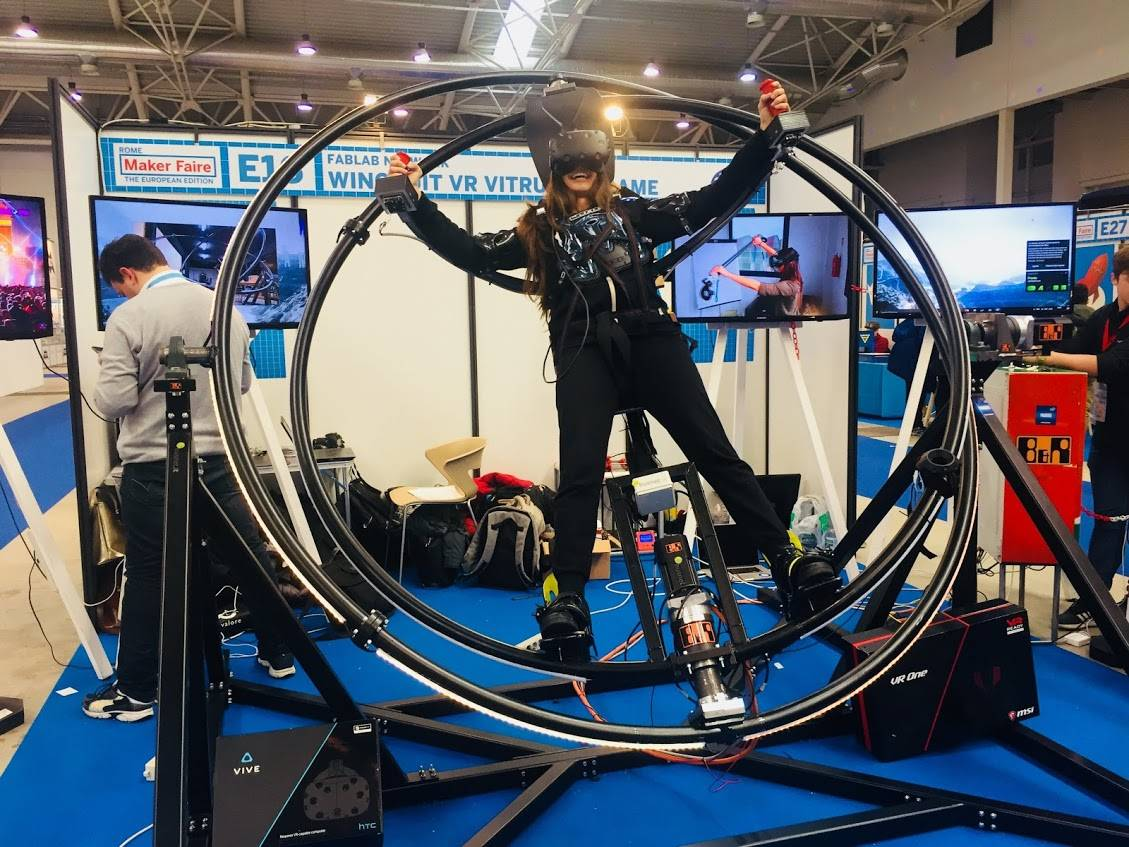
\includegraphics[scale=0.15]{immagini/vitruvian.jpg}
	\caption{Vitruvian Game - Il simulatore di volo con tuta alare}
	\end{center}
\end{figure}

\textbf{FabKey}

FabKey è una serratura smart composta da un sistema di controllo connesso ad internet che permette l'apertura di una porta, andando a verificare una lista di accessi presente in cloud. Funziona tramite lettura di tag \gls{NFC}\textsubscript{G} o barcode. Il prodotto è rivolto principalmente ai \gls{FabLab}, ma si adatta facilmente a qualsiasi contesto in cui sia richiesto il controllo degli accessi.

Le principali tecnologie utilizzate in questo prodotto sono Arduino e relativa programmazione in C/C++ per la parte hardware, mentre per il software crm sono stati utilizzati linguaggi come Html, Javascript, NodeJS, CSS ecc.

\begin{figure}[H]
	\begin{center}
	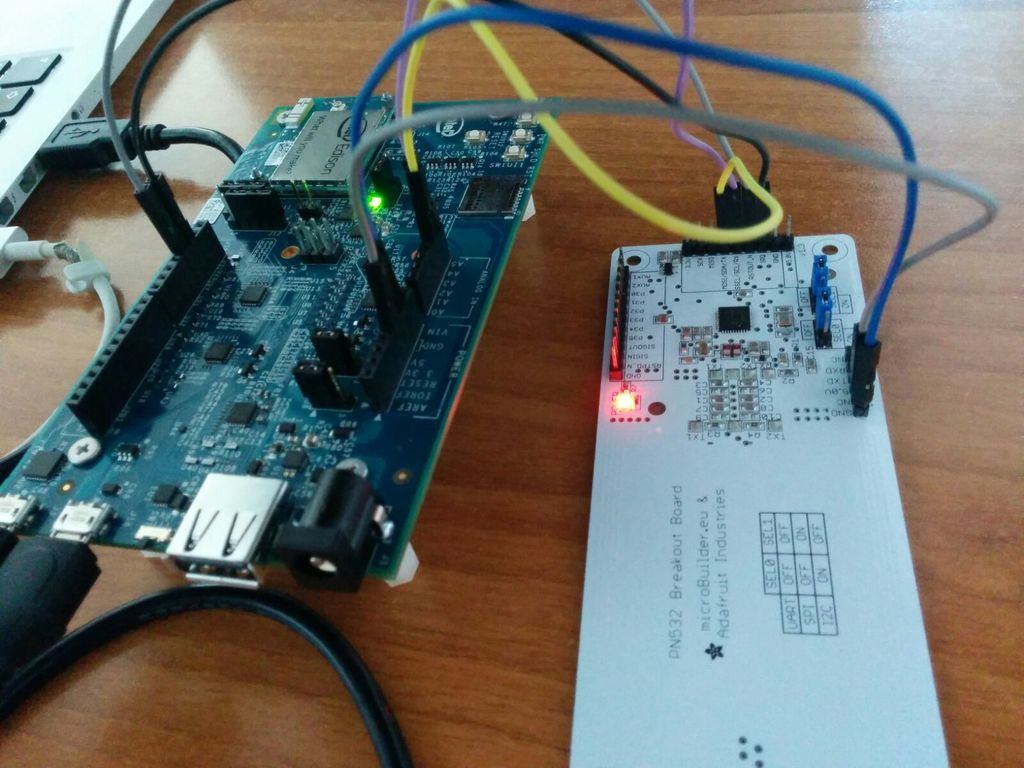
\includegraphics[scale=0.2]{immagini/fabkey.jpg}
	\caption{Prototipo di FabKey durante la fase di programmazione}
	\end{center}
\end{figure}

\textbf{Smart Meter}

Un metro intelligente dotato di rotella metrica ed encoder ottico, capace di misurare superfici complesse e inviare direttamente i dati al software gestionale, in aggiunta anche il monitoraggio in tempo reale di quando, dove e per quanto tempo è stato utilizzato dal singolo addetto.

Il dispositivo è stato sviluppato sulla base di schede elettroniche programmabili open source.

\begin{figure}[H]
	\begin{center}
	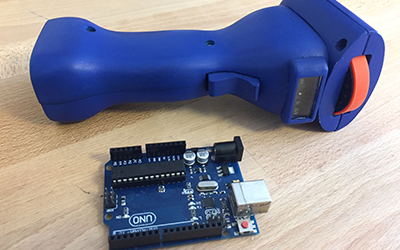
\includegraphics[scale=0.6]{immagini/smartmeter.png}
	\caption{Smart Meter: il metro intelligente}
	\end{center}
\end{figure}

\subsection{Servizi}
Il servizio principale che \lab{} offre ai propri clienti è quello di accompagnare le aziende in un percorso di aggiornamento tecnologico, fornendo supporto in termini di tecnologie e conoscenze.
Durante l'esperienza di stage ho potuto verificare i passaggi che caratterizzano questo servizio:
\begin{itemize}
\item Analisi dettagliata delle esigenze del cliente, tramite diversi incontri con gli stakeholders;
\item Studio di fattibilità grazie ad un'attenta analisi di mercato;
\item Progettazione e/o implementazione dell'innovazione di processo o prodotto lavorando in sinergia con le aziende partner che più si avvicinano alle materie trattate.
\end{itemize}
Altri servizi che \lab{} offre ai propri clienti sono:
\begin{itemize}
\item \textbf{Didattica:} corsi di formazione su misura, \gls{counseling} e \gls{workshop} per imparare a sfruttare in modo professionale: stampa 3D, schede elettroniche, realtà virtuale e aumentata, sviluppo applicazioni, prototipazione, \gls{bigd}, \gls{iot} ecc.
\item \textbf{Noleggio:} kit e attrezzature come stampanti 3D, schede elettroniche (\gls{arduino}, \gls{rpi}, Intel) visori VR, pc e notebook, videoproiettori; affitto di aule didattiche;
\item \textbf{Personale qualificato:} per i clienti sono a disposizione docenti, tecnici di laboratorio e consulenti specializzati nei principali ambiti di innovazione digitale.
\end{itemize}

\subsection{Tecnologie}
L'intero team utilizza ambienti con sistema operativo \textit{macOS} per le attività di sviluppo. 
\subsubsection{Elettronica e Hardware}
A supporto dei processi di prototipazione, \lab{} utilizza diverse piattaforme hardware come ad esempio \textit{Arduino}, \textit{Raspberry Pi}, \textit{Intel UP Square}, \textit{Asus TinkerBoard}.

La programmazione delle schede Arduino avviene tramite l'omonimo ambiente di sviluppo integrato, con linguaggi C/C++.

\lab{}, inoltre, sfrutta le potenzialità della stampa 3D e del disegno CAD per creare modelli prototipali in modo rapido. La disponibilità in azienda di 3 stampanti 3D permette di ridurre il tempo per la realizzazione dei prototipi da proporre al cliente.

Tali tecnologie sono state ampiamente utilizzate per lo sviluppo di progetti come FabKey e SmartMeter, soprattutto in fase di sperimentazione e prototipazione.
\begin{figure}[H]
	\begin{center}
	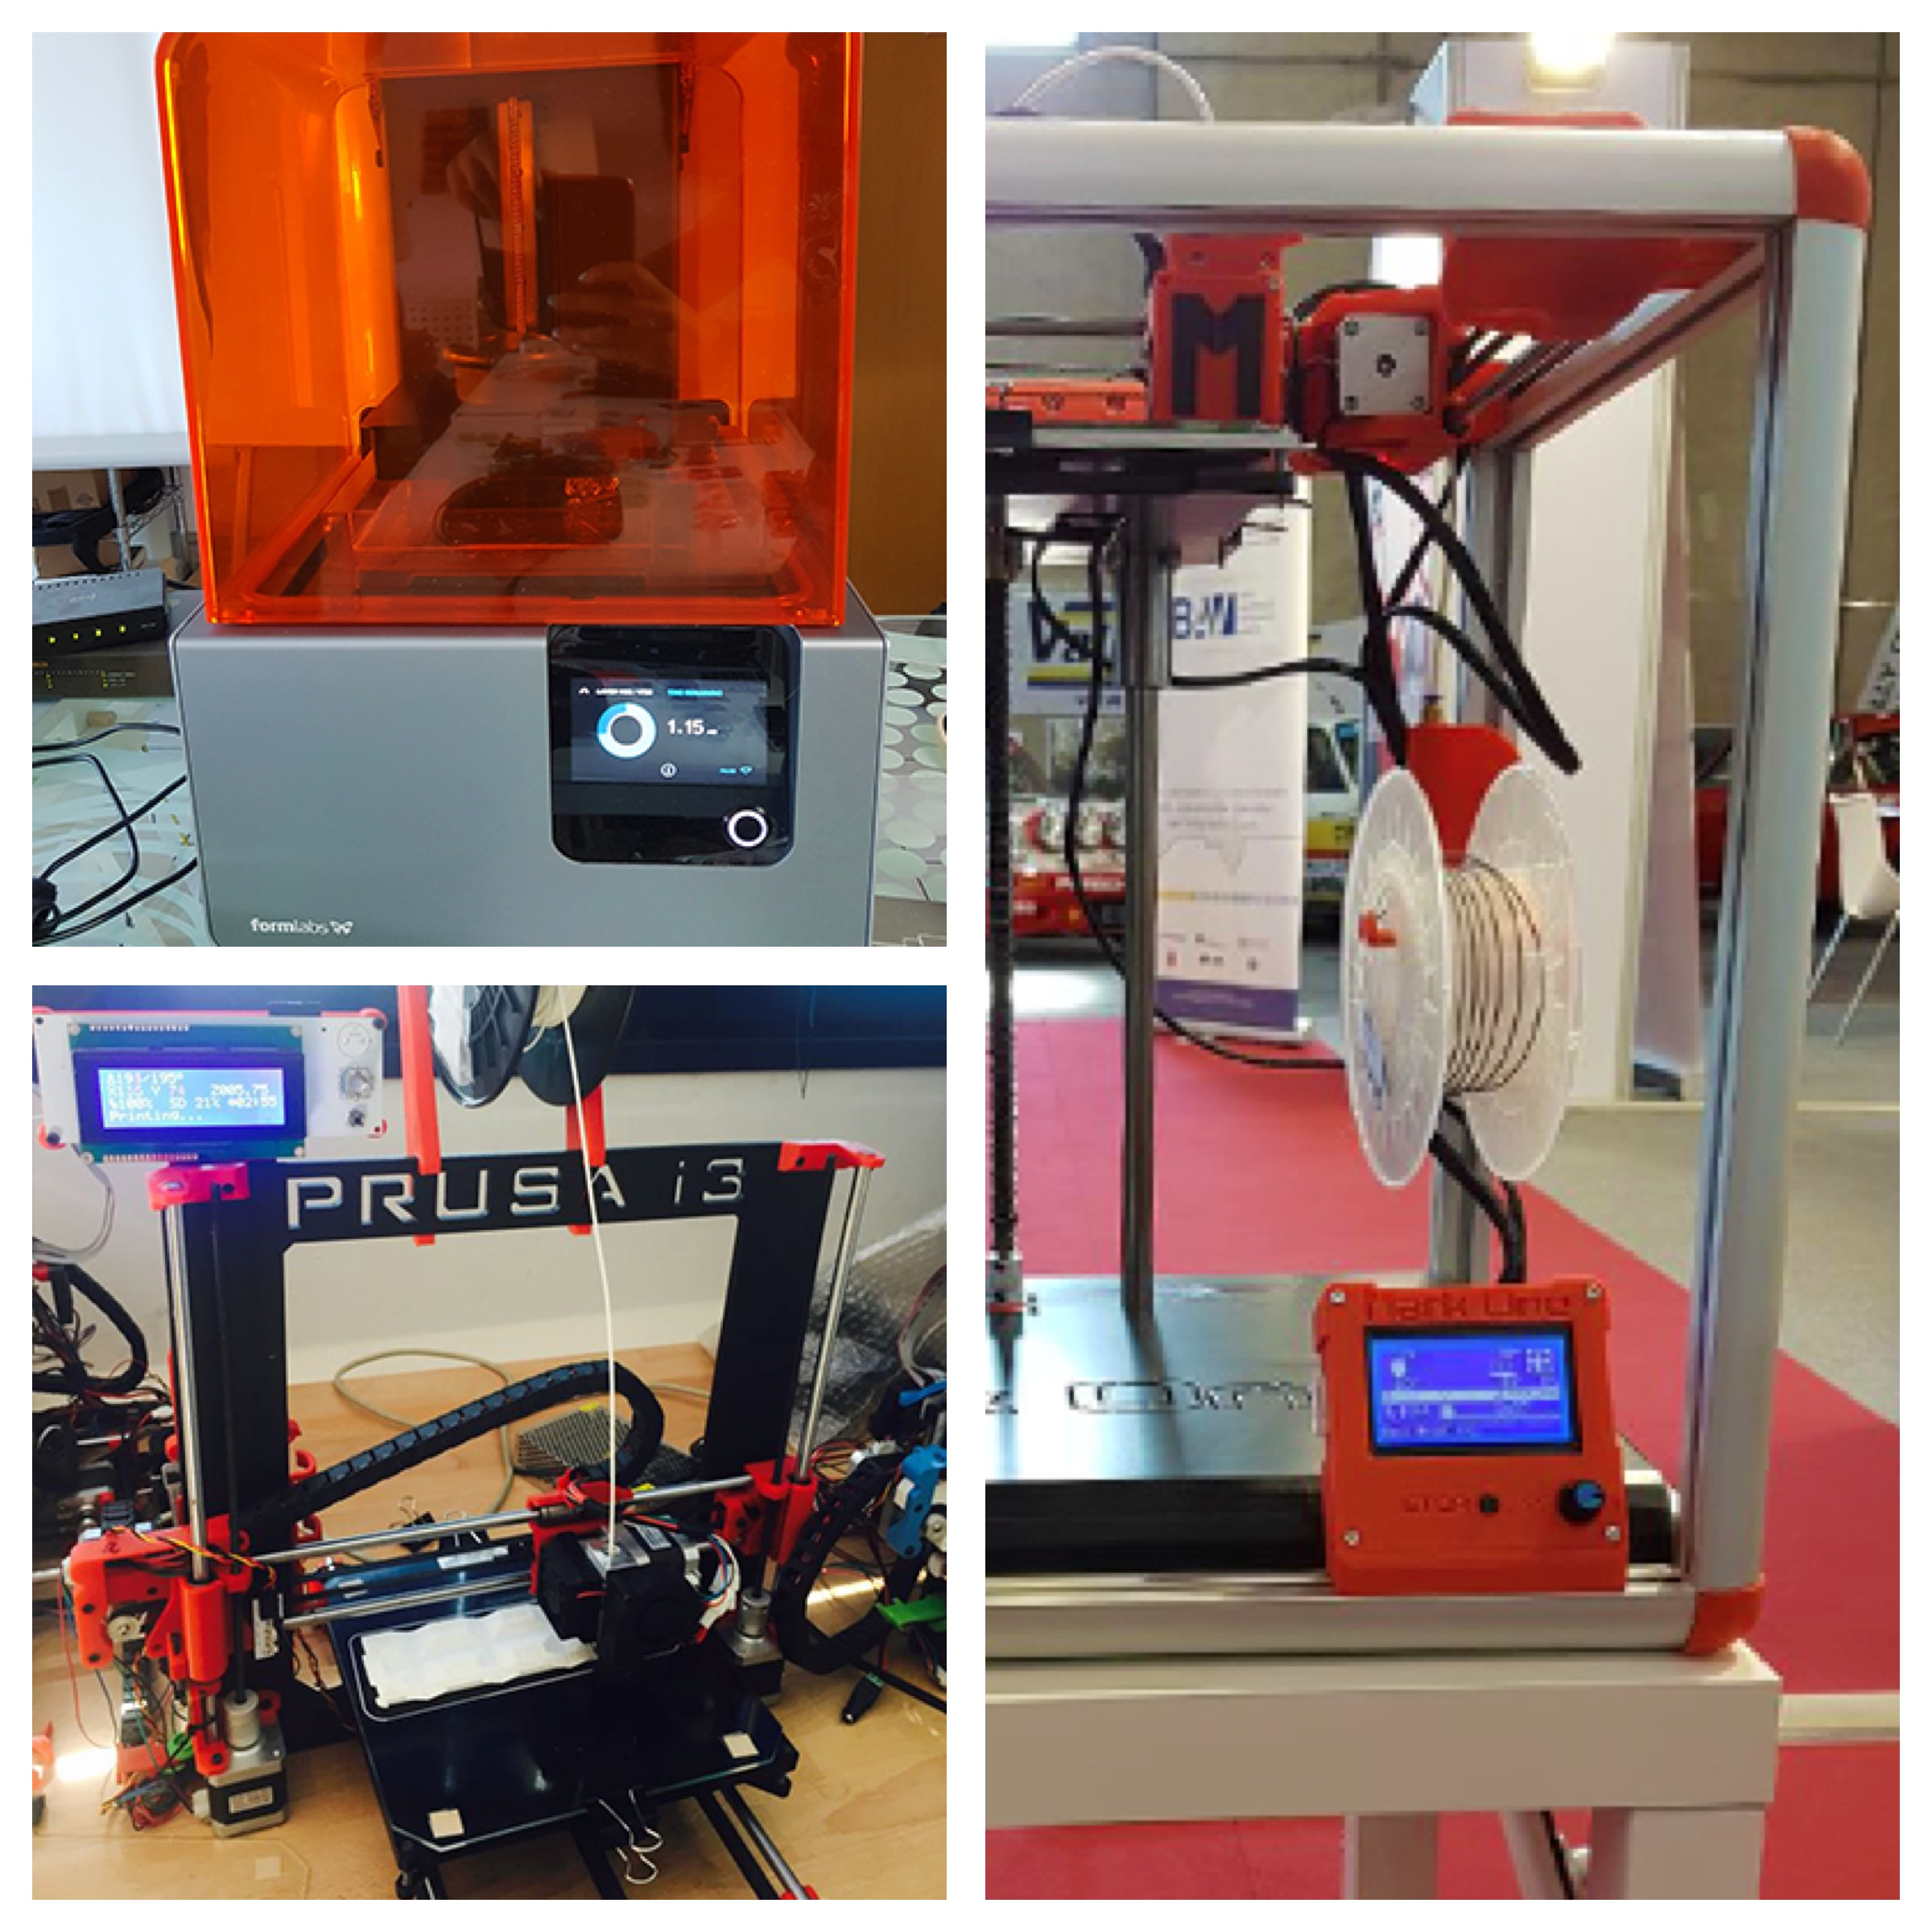
\includegraphics[scale=0.07]{immagini/stampanti.jpg}
	\caption{Le stampanti 3D in dotazione a \lab{}}
	\end{center}
\end{figure}
\subsubsection{Realtà virtuale e aumentata}
L'azienda utilizza software e strumenti per lo studio e lo sviluppo in ambito della realtà virtuale ed aumentata.
Nel dettaglio, è stato utilizzato il motore grafico \textit{Unreal Engine} per lo sviluppo dell'ambiente virtuale relativo al Vitruvian Game: per utilizzare e testare tale ambiente, \lab{} utilizza il visore \textit{Vive} prodotto da \textit{HTC}.

L'azienda, in ambito di realtà aumentata, utilizza la piattaforma \textit{Unity} per lo sviluppo di nuove applicazioni.

\begin{figure}[H]
	\begin{center}
	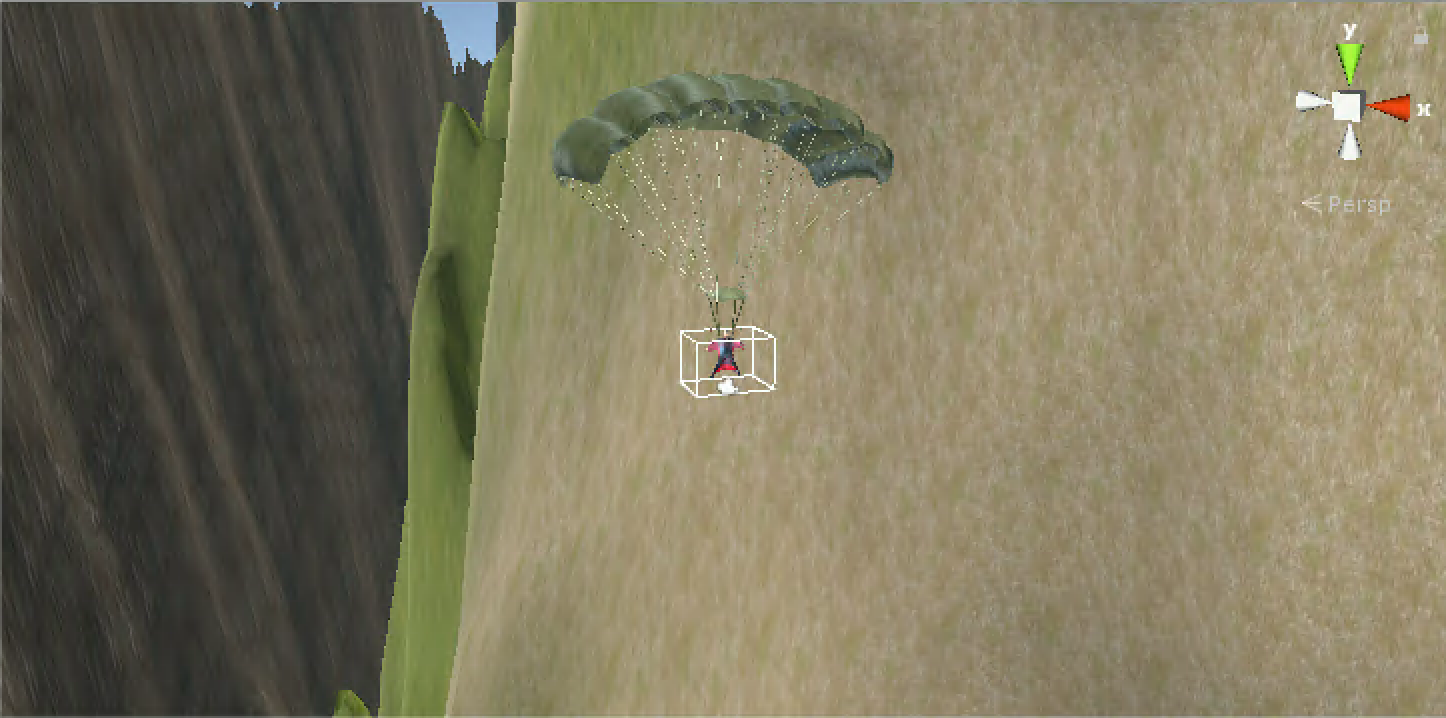
\includegraphics[scale=0.22]{immagini/unity.png}
	\caption{L'ambiente virtuale realizzato con Unreal Engine durante la fase di sviluppo}
	\end{center}
\end{figure}

\subsubsection{Tecnologie di supporto}
A supporto dei processi di sviluppo, l'azienda utilizza la piattaforma web di \textit{GitLab}, che consente la gestione di repository Git e di funzioni trouble ticket.

L'utilizzo di questa piattaforma permette il controllo della configurazione e del versionamento di un software, oltre che la gestione di ticket.

Come detto in precedenza, la piattaforma viene utilizzata anche per la gestione del Product Backlog.

\subsubsection{Sviluppo web}
Alcuni progetti richiedono lo sviluppo di applicazioni web: nel caso di FabKey è stato realizzato un software per la gestione delle autorizzazioni e il controllo degli accessi nei determinati varchi.

Tale applicazione web è stata sviluppata utilizzando PHP e MySQL per la parte backend, mentre HTML, CSS e JavaScript per la parte frontend.

\subsubsection{Deep Learning e intelligenza artificiale}
Intel Movidius è un prodotto di apprendimento profondo che permette di far girare reti neurali profonde in tempo reale direttamente dal dispositivo, consentendo di svolgere un'ampia gamma di applicazioni IA offline.

Utilizzando questa tecnologia, \lab{} sta attualmente sviluppando un progetto che consiste nella previsione di futuri incidenti e infortuni sul lavoro.

Sfruttando le tecniche di \textit{deep learning} messe a disposizione dall'hardware e analizzando grandi dati riguardanti incidenti passati, si è in grado di effettuare una stima sui possibili incidenti futuri.
\begin{figure}[H]
	\begin{center}
	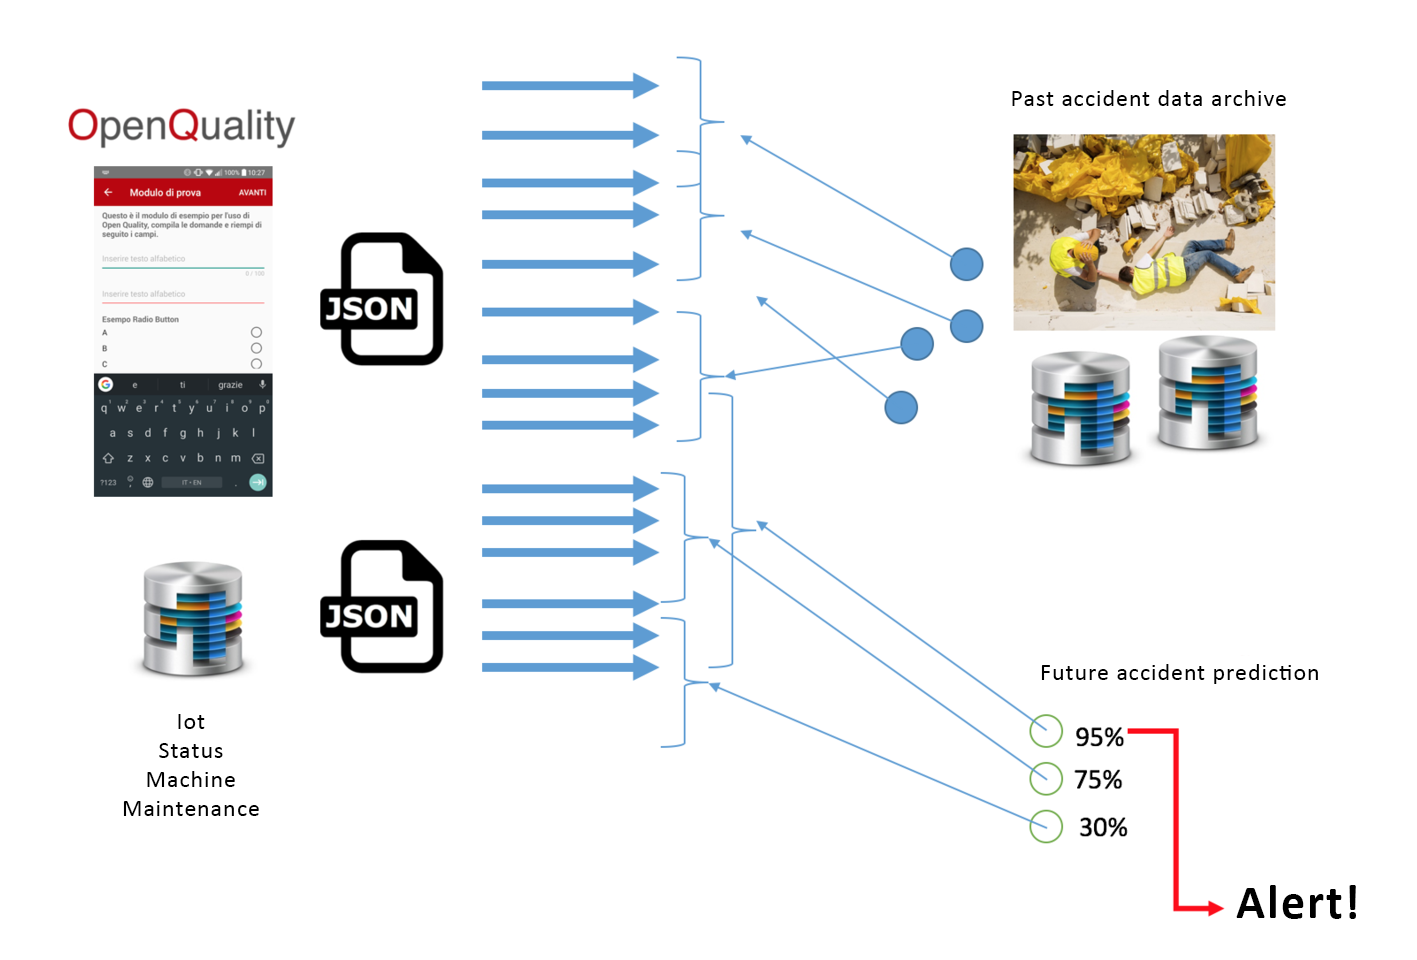
\includegraphics[scale=0.25]{immagini/accident_prediction.png}
	\caption{Previsione degli infortuni sul lavoro: schema di funzionamento}
	\end{center}
\end{figure}

\section{Lab Network e innovazione}
\subsection{Pensiero aziendale}
\lab{} si è sviluppata nell'ambito della \textit{smart specialisation} attraverso logiche di coinvolgimento di una comunità di utenti misti che provengono prevalentemente dal mondo aziendale e accademico. 
L'azienda si propone come punto di riferimento per l'innovazione \textit{Open Source} del Veneto, promuovendosi come centro privilegiato di interscambio di conoscenza.

Come previsto dalla Smart Specialisation Strategy, è stata condotta una prima fase di analisi dall'azienda ed è emerso che il territorio regionale è composto principalmente da piccole e medie imprese di tipo manifatturiero. Sulla base di ciò, \lab{} si è posta l'obiettivo di contribuire, attraverso strumenti e modalità di funzionamento specifici, a sviluppare ed attuare la strategia regionale della ``Fabbrica Intelligente Del Futuro''.

Questa mira ad indirizzare la trasformazione del settore manifatturiero verso nuovi prodotti, processi e tecnologie, attraverso lo sviluppo di attività di ricerca di alto livello.

Per questo \lab{} è sempre alla ricerca di nuove tecnologie, in modo da essere sempre aggiornata 

\subsection{Smart Specialisation Strategy}
\begin{figure}[H]
	\begin{center}
	
\includegraphics[scale=0.15]{immagini/SMART.png}
	\caption{Punti chiave della Smart Specialisation Strategy. Video \textit{"The Kingdom of Smart"}}
	\small{\textbf{Fonte:} \url{http://s3platform.jrc.ec.europa.eu/home}}
	\end{center}
\end{figure}

\begin{flushright}{
	\slshape    
	``L'innovazione non può essere dettata, ma può essere coltivata attraverso scoperte imprenditoriali; ciò richiede una leadership, un impegno comune sostenuto tramite collaborazione e investimenti orientati al futuro.''} 
	
	\medskip
    --- \textit{Pubblicità progresso, Commissione Europea - 2013}
\end{flushright}

% Vedi link: https://www.researchitaly.it/smart-specialisation-strategy/
% Utile: https://www.slideshare.net/TCINetwork/8-clac-18-junefrederic-miribel

\noindent La \textit{Smart Specialisation Strategy} (S.S.S.) è una strategia concepita nell'ambito della politica di coesione riformata dalla Commissione Europea per incentivare l'innovazione regionale al fine di ottenere una crescita economica, permettendo alle regioni di focalizzare i loro punti di forza.

Delinea delle strategie di innovazione concepite a livello regionale ma messe a sistema a livello nazionale con l'obiettivo di:
\begin{itemize}
\item sviluppare strategie di innovazione a livello regionale, mirate a valorizzare ambiti produttivi di eccellenza, considerando il posizionamento strategico all'interno del territorio e le prospettive di sviluppo in un quadro economico globale;
\item aumentare il livello di conoscenza delle Regioni in ambito tecnologico e su settori prioritari;
\item migliorare il modo in cui gli interventi vengono gestiti e governati e aumentare l'efficacia delle attività di valutazione e monitoraggio dei risultati.
\end{itemize}
I passaggi da seguire per attuare questa strategia sono:
\begin{itemize}
\item Analizzare cos'è unico, originale, storico;
\item Definire e condividere una visione per una regione;
\item Definire una priorità ed effettuare una scelta;
\item Trovare l'insieme di politiche migliori da implementare;
\item Selezionare gli indicatori a cui fare riferimento;
\item Istituire una governance;
\item Valutare, rifinire e controllare regolarmente.
\end{itemize}

\begin{figure}[H]
	\begin{center}
	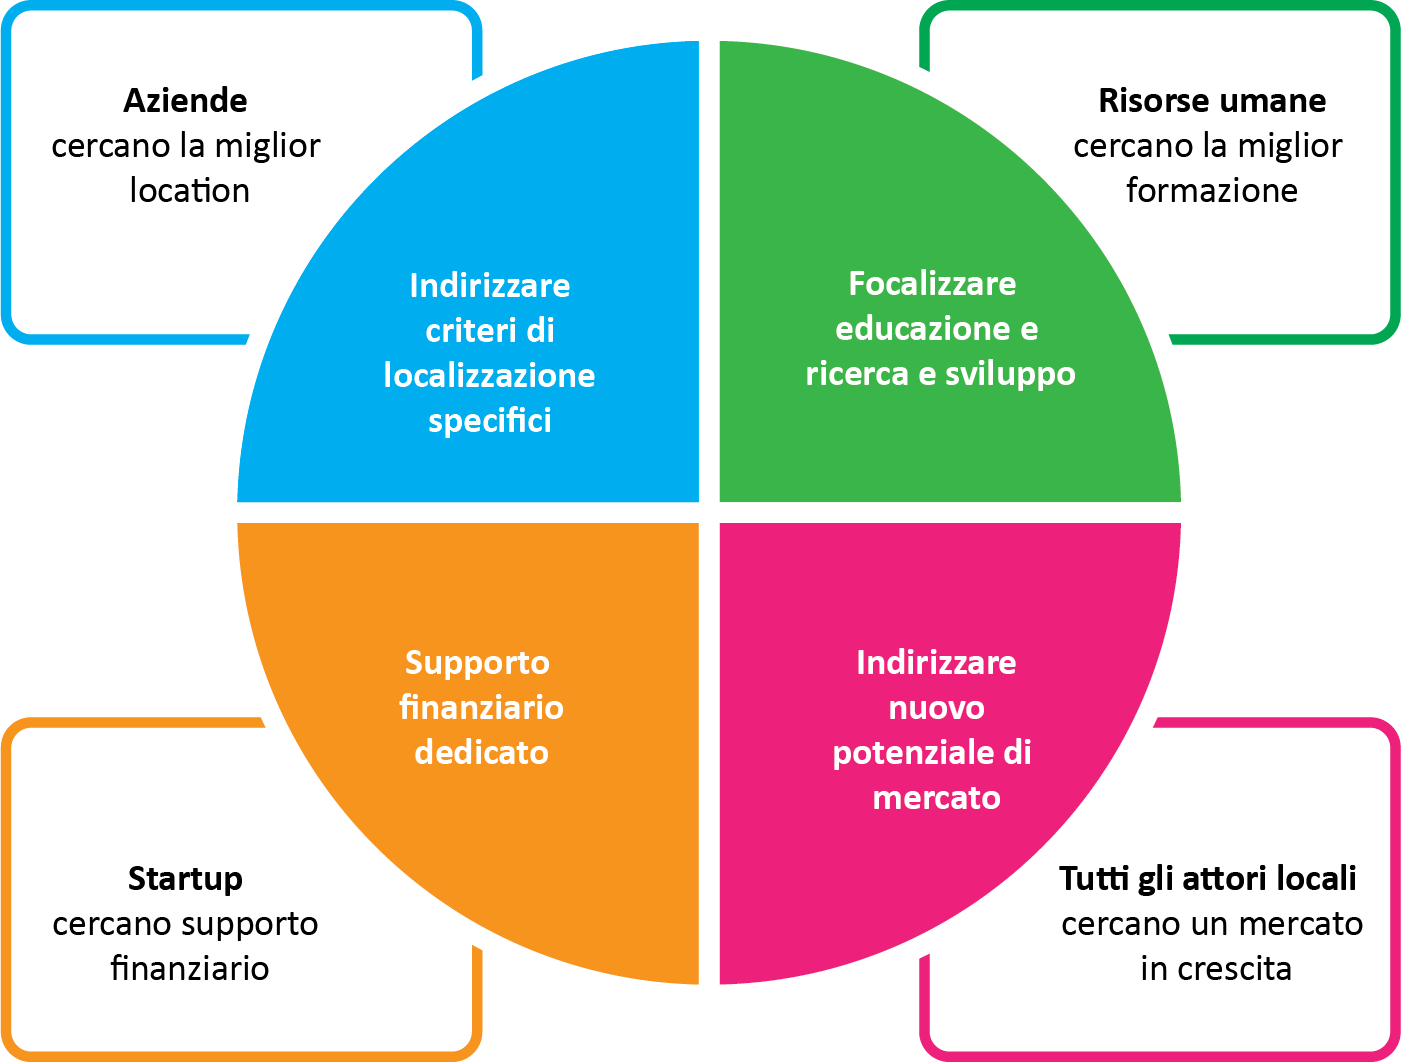
\includegraphics[scale=0.37]{immagini/sss_graph.png}
	\caption{Parti coinvolte e ruoli nella Smart Specialisation Strategy.}
	\small{\textbf{Fonte:} \url{https://www.slideshare.net/TCINetwork/8-clac-18-junefrederic-miribel}}	
	\end{center}
\end{figure}
\subsubsection{L'approccio di Lab Network alla S.S.S.}
\lab{} mette a disposizione un portale dedicato dove aziende e fabbricanti possono comunicare scambiando sapere tecnologico e progetti nell'ottica innovativa dell'economia condivisa.

L'\gls{SWOT} (Strengths, Weakness, Opportunities, Threats) condotta da \lab{} sulla realtà delle PMI venete, evidenzia come ci sia uno scarso utilizzo di tecnologie dell'informazione e della comunicazione (ICT), scarsa disponibilità di laboratori di proprietà, bassi investimenti in ricerca, difficoltà a sviluppare progetti innovativi e ridotta capacità di reperire risorse e professionalità necessarie. 
L'obiettivo di \lab{} è quello di colmare queste lacune mettendo a disposizione alle aziende un'area di lavoro a costi contenuti dove poter utilizzare i principali strumenti di innovazione digitale come: stampanti 3D, kit elettronici, macchine a controllo numerico, frese digitali e taglio laser. Tutto questo può essere definito come un laboratorio per studiare la fase prototipale.

In pratica \lab{} vuole contribuire a portare l'innovazione e la tecnologia all'interno delle PMI che ancora non si sono interfacciate a questo ``nuovo mondo''.
\newpage             % Contesto aziendale
% !TEX encoding = UTF-8
% !TEX TS-program = pdflatex
% !TEX root = ../tesi.tex

%**************************************************************
\chapter{Il progetto nella strategia aziendale}
\label{cap:processi-metodologie}
%**************************************************************

\section{Azienda e stage}
Lab Network Srl è solita ospitare tirocinanti e stagisti per dare loro una formazione e valutarne le capacità per un possibile inserimento in azienda.

Il tirocinio porta un vantaggio sia per gli stagisti stessi, che hanno modo di mettere in pratica in campo lavorativo quanto appreso durante gli studi, sia per l'azienda che ha modo di valutare le capacità di una persona al fine dell'assunzione formandola al tempo stesso. Gli stage offrono inoltre la possibilità all'azienda di avviare progetti che normalmente non avrebbero spazio. 

Sono venuto a conoscenza di Lab Network grazie alla diffusione mediatica di alcuni loro progetti che stavano avendo successo, come ad esempio Vitruvian Game, così ho deciso quindi di propormi all'azienda per lo svolgimento del tirocinio: Lab Network ha accettato proponendomi alcuni progetti disponibili tra cui FabKey.

Lab Network ha deciso di portare avanti questo progetto attraverso uno stage, perché fino ad allora era stato catalogato come secondario e non aveva ancora trovato il suo spazio all'interno dell'azienda.

\section{Obiettivi aziendali}
L'obiettivo principale del progetto di stage è l'ampliamento del già collaudato sistema ``FabKey'', il quale permette l'apertura di una porta attraverso un tag NFC controllando una lista di accessi presente in un database online. Nello specifico, tale sistema doveva essere revisionato e ampliato, utilizzando un modulo che andrà ad autenticare l'utente tramite codice a barre anziché tag NFC.

Gli obiettivi concordati con il tutor aziendale sono stati classificati secondo tre gradi di priorità:

\begin{enumerate}
\item \textbf{Obbligatori}: obiettivi il cui sviluppo è necessario per la riuscita del progetto;
\begin{itemize}
\item \textbf{Integrazione di un sistema completo per l'apertura di serrature con lettura di codice a barre e NFC.} L'obiettivo principale richiesto dall'azienda è quello di ampliare il sistema esistente, che consiste in una centralina di controllo e di un modulo NFC, con un modulo per la lettura di codici a barre. Si rende necessaria la riprogrammazione della centralina, aggiungendo la nuova parte di codice per la gestione dei codici a barre; 
\item \textbf{Realizzazione della piattaforma web per la gestione degli accessi.} La piattaforma web per il controllo degli accessi è uno strumento indispensabile per l'utilizzo del sistema FabKey, pertanto la sua realizzazione è un requisito obbligatorio. Questa applicazione web sarà composta da un pannello di controllo che permette l'utente di modificare le autorizzazioni d'accesso a uno o più varchi e di consultare un report contenente tutti gli accessi effettuati; 
\item \textbf{Creazione del modello 3D dell'involucro e sua realizzazione con stampa 3D.} Durante la definizione degli obiettivi è stato accordato che tutta la parte elettronica avrà alloggiamento in un involucro disegnato su misura e stampato in 3D; 
\item \textbf{Redazione della manualistica completa.} A corredo del kit, all'utente finale andrà consegnata tutta la manualistica necessaria all'installazione e all'uso. Sono necessari anche dei manuali interni per la guida all'assemblaggio, alla codifica e alla corretta configurazione per il cliente finale;
\end{itemize}
\item \textbf{Desiderabili}: il loro sviluppo non è necessario ai fini del progetto, ma forniscono un valore aggiunto considerevole;
\begin{itemize}
\item \textbf{Cura e definizione dell'interfaccia grafica della piattaforma web.} Seppur trattandosi di un aspetto non vincolante ai fini del progetto, una grafica curata fornisce ottimo valore aggiunto al prodotto finale;
\item \textbf{Ottimizzazione del sistema esistente in termini di efficienza e prestazioni}. Con questo obiettivo si vogliono ridurre i tempi di risposta dell'intero sistema ottimizzando l'esecuzione del codice in generale e in particolare le chiamate HTTP al server; 
\end{itemize}
\item \textbf{Facoltativi}: il loro sviluppo diventa apprezzabile, ma dal valore aggiunto trascurabile.
\begin{itemize}
\item \textbf{Creazione di un modello 3D modulare espandibile per future versioni}. In previsione di future espansioni con l'utilizzo di elettronica differente, è apprezzabile la creazione del modello 3D in modo modulare e universale, compatibile quindi con eventuali modifiche future. 
\end{itemize}
\end{enumerate}

\section{Vincoli}
Mi sono stati imposti dei vincoli da parte dell'azienda in termini di tempo e tecnologie al fine di un corretto svolgimento del progetto oltre che una buona integrazione con il resto del team di sviluppo. Quanto stabilito a monte dello stage, è stato trascritto all'interno di un piano di lavoro, redatto in collaborazione con il tutor aziendale.

I vincoli tecnologici sono:
\begin{itemize}
\item \textbf{GitLab}: si tratta di una piattaforma web per la gestione di repository Git. Mi è stato chiesto di utilizzare questo strumento anche per la gestione di ticket e del Product Backlog;
\item \textbf{Arduino IDE}: applicazione che consente la programmazione di schede Arduino e compatibili. Viene fornito con un editor di testo, un compilatore e una serie di esempi per ogni libreria disponibile.
\item \textbf{Rhinoceros}: software per la modellazione 3D, mi è stato chiesto, dopo un'adeguata documentazione, di utilizzarlo per la modellazione dell'involucro contenente l'elettronica di FabKey.
\end{itemize}

Il tempo a disposizione per lo svolgimento dello stage è di almeno 300 ore, le quali sono state suddivise in 40 ore settimanali per le prime 5 settimane e le rimanenti ore suddivise su una base di 24 ore settimanali.

\section{Obiettivi personali}
Le mie aspettative prima dello svolgimento dello stage presso \lab{} erano:
\begin{itemize}
\item Imparare la programmazione di schede open source come Arduino affacciandomi quindi al mondo dell'IOT in forte espansione;
\item Capire a fondo il principio di funzionamento della stampa 3D, conoscere le varie problematiche e relative soluzioni; parallelamente apprendere le basi per la modellazione 3D
\item Riuscire a lavorare in un team di sviluppo 
\end{itemize}

\begin{itemize}
\item \textbf{Codifica e correlazione tra hardware e software}: un aspetto dell'informatica che mi ha da sempre affascinato è la relazione tra hardware e software; non avendo potuto approfondire l'argomento durante gli studi, ho trovato questa proposta di stage un'ottima opportunità per studiare sul campo la programmazione hardware. Il progetto, inoltre, si affaccia al mondo dell'\textit{Internet Of Things} che è in continua crescita;
\item \textbf{Modellazione e stampa 3D}: campo molto diffuso e in continua crescita è quello della stampa 3D: con questo progetto di stage mi è stata offerta la possibilità di usare in esclusiva una stampante 3D per la realizzazione dei primi prototipi dopo averli correttamente modellati;
\item \textbf{Lavoro in team}: fare parte di un team di sviluppo cogliendo gli aspetti in comune e le differenze tra un progetto accademico come quello svolto durante il corso di Ingegneria del Software e un progetto in ambito lavorativo.
\end{itemize}

             % Il progetto nella strategia aziendale
% !TEX encoding = UTF-8
% !TEX TS-program = pdflatex
% !TEX root = ../tesi.tex

%**************************************************************
\chapter{Lo stage}
\label{cap:descrizione-stage}
%**************************************************************

\section{Pianificazione}
Prima dell'inizio del progetto, ho redatto assieme al tutor aziendale un piano di lavoro, all'interno del quale ho riportato gli obiettivi individuati, la pianificazione del lavoro sotto forma di processi, suddivisi a loro volta in attività, ad ognuna delle quali sono state assegnate delle ore di lavoro, la cui somma sarà il totale delle ore a disposizione per lo stage.

\bigskip

%% !TEX encoding = UTF-8
% !TEX TS-program = pdflatex
% !TEX root = ../tesi.tex

% Tabella da personalizzare in base alle ore delle attività

\begin{tabularx}{\textwidth}{|c|X|}
	\hline
	\textbf{Durata in ore} & \textbf{Descrizione dell'attività} \\\hline
	
	\textbf{48} & \textbf{Formazione sulle tecnologie utilizzate} \\	 
    \hline
    
    \textbf{72} & \textbf{Definizione del sistema hardware/software e relativa documentazione} \\ \hdashline 
    \multirow{3}{0cm}\\ 
    \textit{16} & 
    \textit{Analisi del problema e del dominio applicativo} \\
    \textit{26} & 
    \textit{Adattamento e revisione della piattaforma esistente} \\
    \textit{8} & 
    \textit{Test piattaforma hardware} \\
    \textit{18} & 
    \textit{Progettazione e sviluppo software CRM} \\
    \textit{4} & 
    \textit{Stesura documentazione} \\
    \hline
    
    \textbf{24} & \textbf{Modellazione e Stampa 3D}  \\ \hdashline 
    \multirow{4}{0cm}\\ 
    \textit{18} & 
    \textit{Design e modellazione involucro} \\
    \textit{6} & 
    \textit{Slicing del modello e stampa 3D} \\
    \hline
    
    \textbf{48} & \textbf{Sviluppo piattaforma online}  \\ \hdashline 
    \multirow{4}{0cm}\\ 
    \textit{18} & 
    \textit{Pianificazione e analisi dei requisiti} \\
    \textit{30} & 
    \textit{Sviluppo della piattaforma con iniziale attenzione al lato server} \\
    \hline
    
    \textbf{40} & \textbf{Cura dell'interfaccia grafica}  \\ 
    \hline
    
    \textbf{16} & \textbf{Test e verifica presenza bug}  \\
    \hline
    
	\textbf{48} & \textbf{Redazione dei manuali d'uso}  \\
    \hline    
    
    \textbf{12} & \textbf{Collaudo Finale}  \\ \hdashline 
    \multirow{4}{0cm}\\ 
    \textit{8} & 
    \textit{Collaudo} \\
    \textit{2} & 
    \textit{Incontro di presentazione della piattaforma con gli stakeholders} \\
    \textit{2} & 
    \textit{Live demo di tutto il lavoro di stage} \\
    \hline
	
	\textbf{Totale ore} & \multicolumn{1}{|c|}{\textbf{\totaleOre}} \\\hline
	
	
\end{tabularx} % tolta tabella in quanto sotto ho omesso la voce "Progettazione e sviluppo software CRM"

%\medskip

%DIAGRAMMA DI GANTT???

%\medskip

Le attività individuate sono:
\begin{itemize}
\item \textbf{Formazione sulle tecnologie utilizzate}: la fase iniziale dello stage consiste nella formazione sulle tecnologie usate, oggetto dei vincoli posti dall'azienda. Questa è stata una fase molto importante per poter lavorare correttamente ed in sincronia con il resto del team;

\item \textbf{Definizione del sistema hardware/software e relativa documentazione}
\begin{itemize}
	\item \textbf{Analisi del problema e del dominio applicativo}: la prima attività da svolgere è stata quella di analizzare il problema e il contesto in cui il prodotto dovrà operare. Questa attività include anche lo studio del sistema esistente in modo da comprenderne in modo esaustivo il funzionamento. Come prodotto in uscita ho ottenuto tutti i requisiti relativi alla parte hardware del progetto;
	\item \textbf{Adattamento e revisione della piattaforma esistente}: una volta compreso il funzionamento del sistema esistente e formalizzato i requisiti ottenuti dall'attività precedente, ho progettato la modifica da apportare per poter lavorare con il nuovo modulo ed in seguito ho riportato il tutto su codice;
	\item \textbf{Test piattaforma hardware}: ho pianificato ed eseguito alcuni test d'unità che andassero a verificare la correttezza sulle nuove parti di codice;
	\item \textbf{Stesura documentazione}: per poter garantire un'adeguata manutenzione al prodotto, ho redatto in questa attività tutta la documentazione relativa alle nuove modifiche;
\end{itemize}

\item \textbf{Modellazione e Stampa 3D}
\begin{itemize}
	\item \textbf{Design e modellazione involucro}: ho dedicato del tempo per la creazione digitale del modello tridimensionale per l'involucro che conterrà l'elettronica del nuovo modulo aggiunto;
	\item \textbf{Slicing del modello e stampa 3D}: ho preparato il modello creato nell'attività precedente per la stampa andando ad impostare vari parametri al computer ed infine ho provveduto alla stampa vera e propria;
\end{itemize}

\item \textbf{Sviluppo piattaforma online}
\begin{itemize}
	\item \textbf{Pianificazione e analisi dei requisiti}: ho pianificato e analizzato i requisiti per lo sviluppo della piattaforma online. Questo strumento serve al cliente finale per monitorare i vari accessi al varco controllato da FabKey e per gestire gli accessi autorizzati;
	\item \textbf{Sviluppo della piattaforma con iniziale attenzione al lato server}: a seguito della pianificazione e raccolta dei requisiti, ho proseguito con lo sviluppo della piattaforma, con priorità al lato server;
\end{itemize}

\item \textbf{Cura dell'interfaccia grafica}: ho prestato attenzione alla cura dell'interfaccia grafica relativa alla piattaforma creata nelle attività precedenti. Durante questa attività ho curato anche la parte front-end dell'applicazione online;
\item \textbf{Test e verifica presenza bug}: al termine della fase di sviluppo ho eseguito dei test sul sistema completo;
\item \textbf{Redazione dei manuali d’uso}: in questa attività ho redatto tutti i manuali d'uso sia per l'utente (uso e installazione del sistema), sia per uso interno (assemblaggio e configurazione del sistema);

\item \textbf{Collaudo Finale}
\begin{itemize}
	\item \textbf{Collaudo}: collaudo finale prima della presentazione ufficiale;
\end{itemize}
\end{itemize}

\medskip

Ho riportato gli obiettivi individuati sul piano di lavoro, categorizzandoli secondo tre tipologie come spiegato nella sezione 2.2


%**************************************************************
\section{Studio iniziale}
\subsection{Documentazione individuale}
Gli obiettivi e i vincoli fissati comprendevano alcune tecnologie e strumenti che ancora non facevano parte del mio bagaglio formativo, pertanto lo stage ha avuto inizio con una fase di studio individuale.
Supportato dal tutor aziendale e dai colleghi, ho iniziato lo studio degli strumenti che l'azienda usa regolarmente durante lo sviluppo di un progetto, come GitLab, la piattaforma online per repository Git. In precedenza, durante alcuni progetti universitari, tra i quali quello di Ingegneria del Software, ho utilizzato il software di versionamento Git tramite la piattaforma di GitHub, simile per molti aspetti a GitLab. Per questo l'apprendimento non è stato difficile.

\medskip

Ha richiesto più tempo lo studio del software di modellazione 3D Rhinoceros. Non essendomi mai approcciato al disegno e modellazione tridimensionale, apprendere le basi è stata un'operazione più lunga del previsto, ma, una volta compreso il principio alla base, la creazione di modelli semplici è un processo abbastanza semplice.

Ho avuto la possibilità di studiare il funzionamento della stampa 3D grazie alla disponibilità di una stampante a mio uso esclusivo. Ciò mi ha permesso di effettuare diversi test modificando i parametri di stampa e sperimentando diversi materiali, il tutto prima dello sviluppo del progetto.

\medskip

L'ultimo strumento oggetto di studio è stato Arduino. Ho iniziato studiando l'editor e le modalità di collegamento alla scheda. Prima di iniziare con dei test di funzionamento, ho preferito utilizzare il software Fritzing\footcite{http://fritzing.org/} per disegnare gli schemi di collegamento dei componenti elettronici alla scheda; questo strumento si è reso utile anche durante la redazione dei manuali ad uso interno per la guida all'assemblaggio.

\begin{figure}[H]
	\begin{center}
	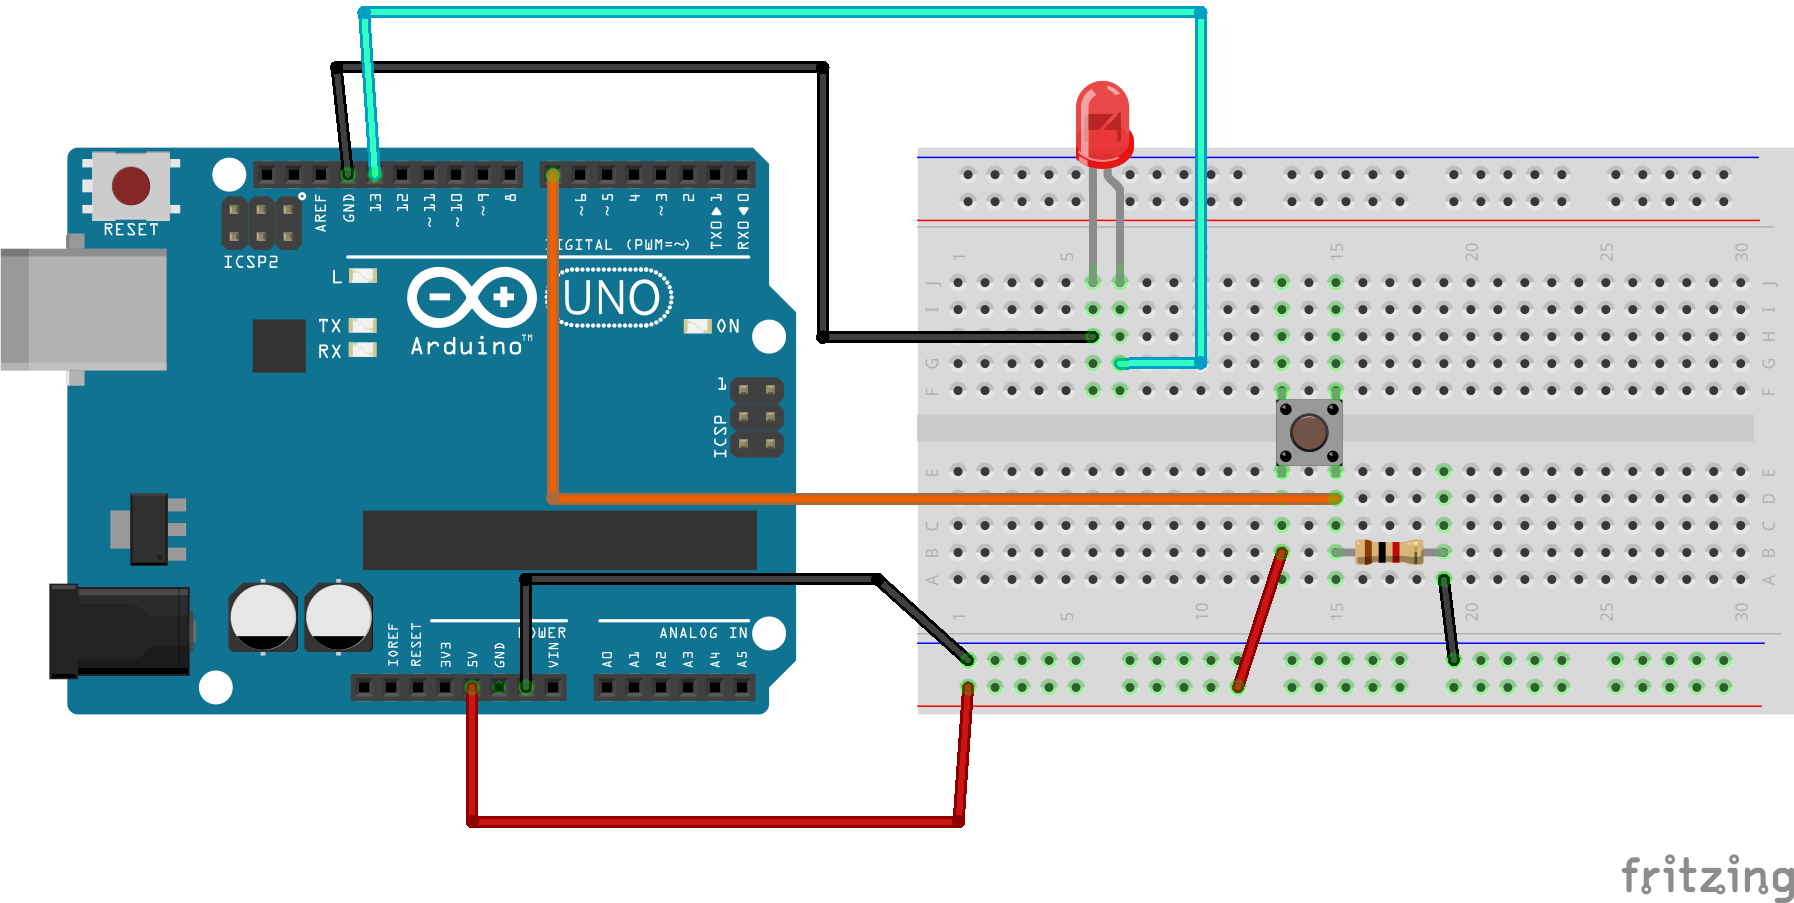
\includegraphics[scale=0.62]{immagini/schema_arduino.png}
	\caption{Esempio di schema creato con Fritzing. Rappresenta uno dei primi test effettuati con scheda Arduino.}
	\end{center}
\end{figure}

\medskip

%Il progetto verrà spiegato in questa sezione, senza però scendere in dettagli, evitando quindi riproducibilità.
Lo sviluppo del progetto è partito da uno studio preliminare sul sistema già esistente composto da una centralina di controllo ed un lettore di schede NFC.
Scendendo nei dettagli, la fase di studio è iniziata dalla centralina, composta da una scheda Arduino. Per poterne apprendere il funzionamento, il tutor aziendale mi ha fornito una scheda di test sulla quale eseguire del codice di esempio con dei semplici circuiti elettronici. L'apprendimento si è rivelato piuttosto rapido anche grazie alla vasta disponibilità di materiale online e ad una consolidata community.

Una volta appreso il funzionamento generale di Arduino, ho iniziato lo studio sul codice che governa il comportamento della centralina di controllo, caratterizzato principalmente da 3 fasi:

\begin{itemize}
\item \textbf{Configurazione iniziale}: il sistema esegue una configurazione iniziale in modo da integrarsi perfettamente nella rete alla quale è collegato;
\item \textbf{Listener}: una porzione di codice che rimane in continuo ascolto per catturare gli eventi derivanti dai moduli collegati;
\item \textbf{Crittografia e HTTP request}: una funzione che si occupa della cifratura dei codici letti e del loro invio tramite richieste HTTP ad un server.
\end{itemize}

Terminata questa prima fase di studio, è susseguita quella di analisi.

\section{Analisi dei requisiti}
\subsection{Identificazione}
Per poter identificare correttamente tutti i requisiti, a seguito di vari colloqui con il tutor aziendale e il cliente, ho definito i vari casi d'uso, disegnandone in seguito i rispettivi diagrammi UML. Ogni riunione è stata riportata su di un verbale e da quest'ultimo ho in seguito ricavato i vari requisiti. Ho anche analizzato approfonditamente i casi d'uso in modo da poter identificare ulteriori requisiti. Una volta individuati tutti i requisiti sono stati riportati in un documento soggetto a versionamento.

\subsection{Strumenti a supporto}
\subsubsection{Casi d'uso}
I casi d'uso e i relativi diagrammi UML sono stati un ottimo strumento di supporto durante la fase di analisi: mi hanno permesso di individuare alcuni requisiti non emersi durante le riunioni con tutor e stakeholders.

\begin{figure}[H]
	\begin{center}
	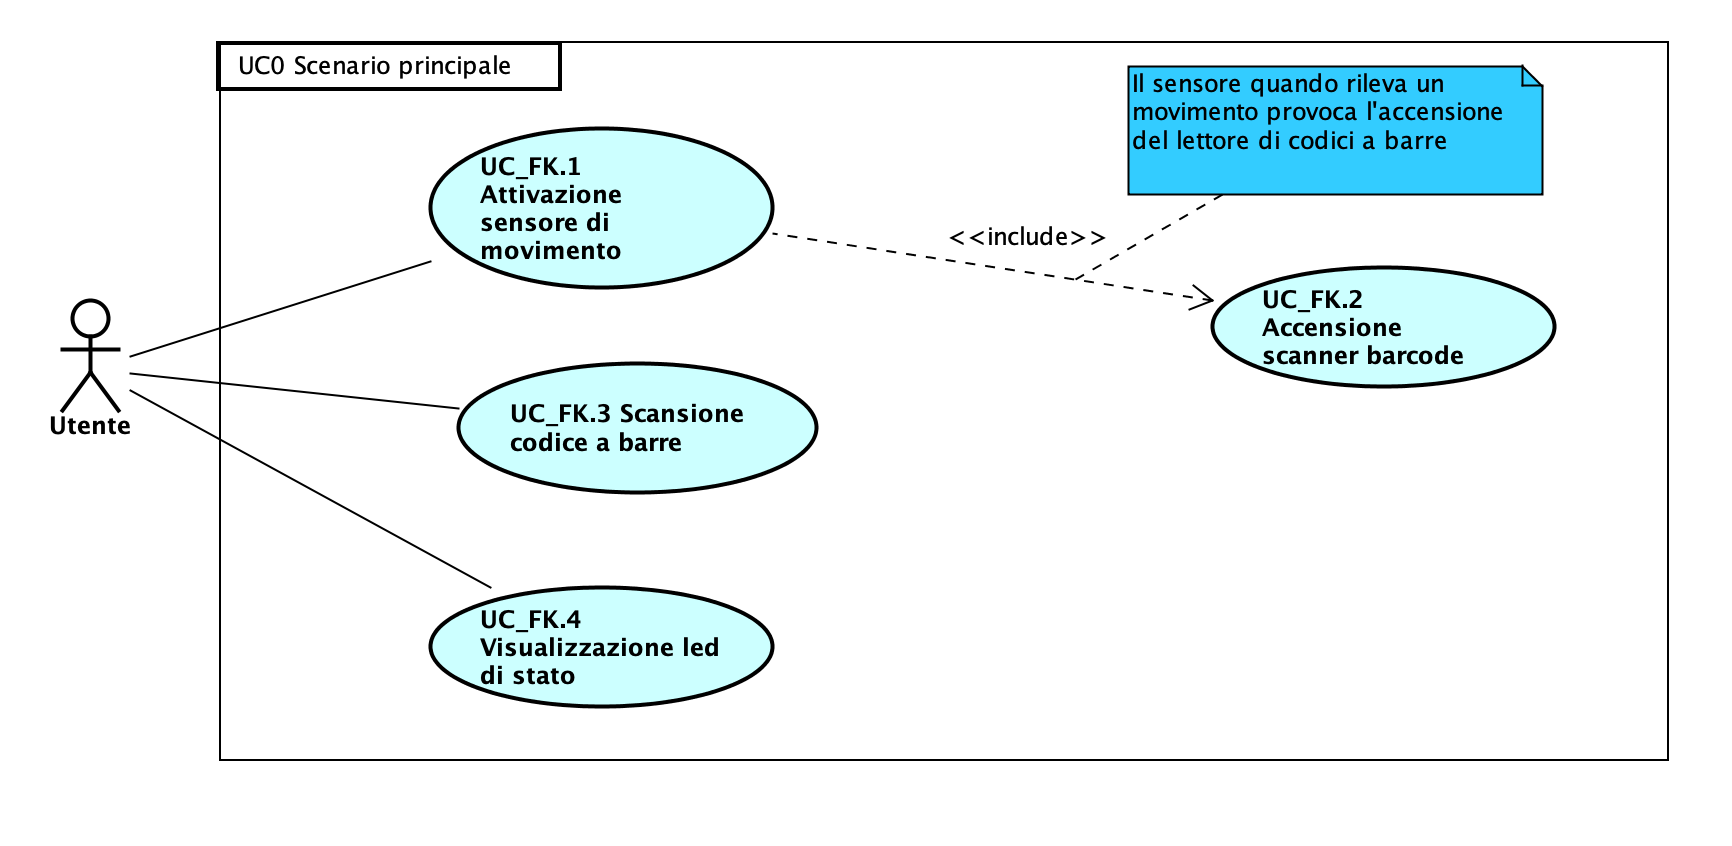
\includegraphics[scale=0.4]{immagini/usecase/scenario_principale.png}
	\caption{Estratto dello schema UML rappresentante i casi d'uso dello scenario principale. Schema riferito all'uso di FabKey e non alla piattaforma online.}
	\end{center}
\end{figure}

Essendo il progetto composto da due sistemi, FabKey e piattaforma online, i casi d'uso sono stati categorizzati da una notazione univoca, che facilita l'identificazione del caso d'uso nel contesto:

\begin{center}
\textbf{UC\textunderscore [Contesto].[IDUnivoco]}
\end{center}

\begin{itemize}
\item \textbf{Contesto}:
\begin{itemize}
\item \textbf{FK}: FabKey;
\item \textbf{PO}: Piattaforma online di gestione.
\end{itemize}

\item \textbf{IDUnivoco}: Un codice numerico progressivo che identifica in maniera univoca il caso d'uso a cui si riferisce. Questo codice può essere gerarchico in modo da identificare casi d'uso innestati.
\end{itemize}

\begin{figure}[H]
	\begin{center}
	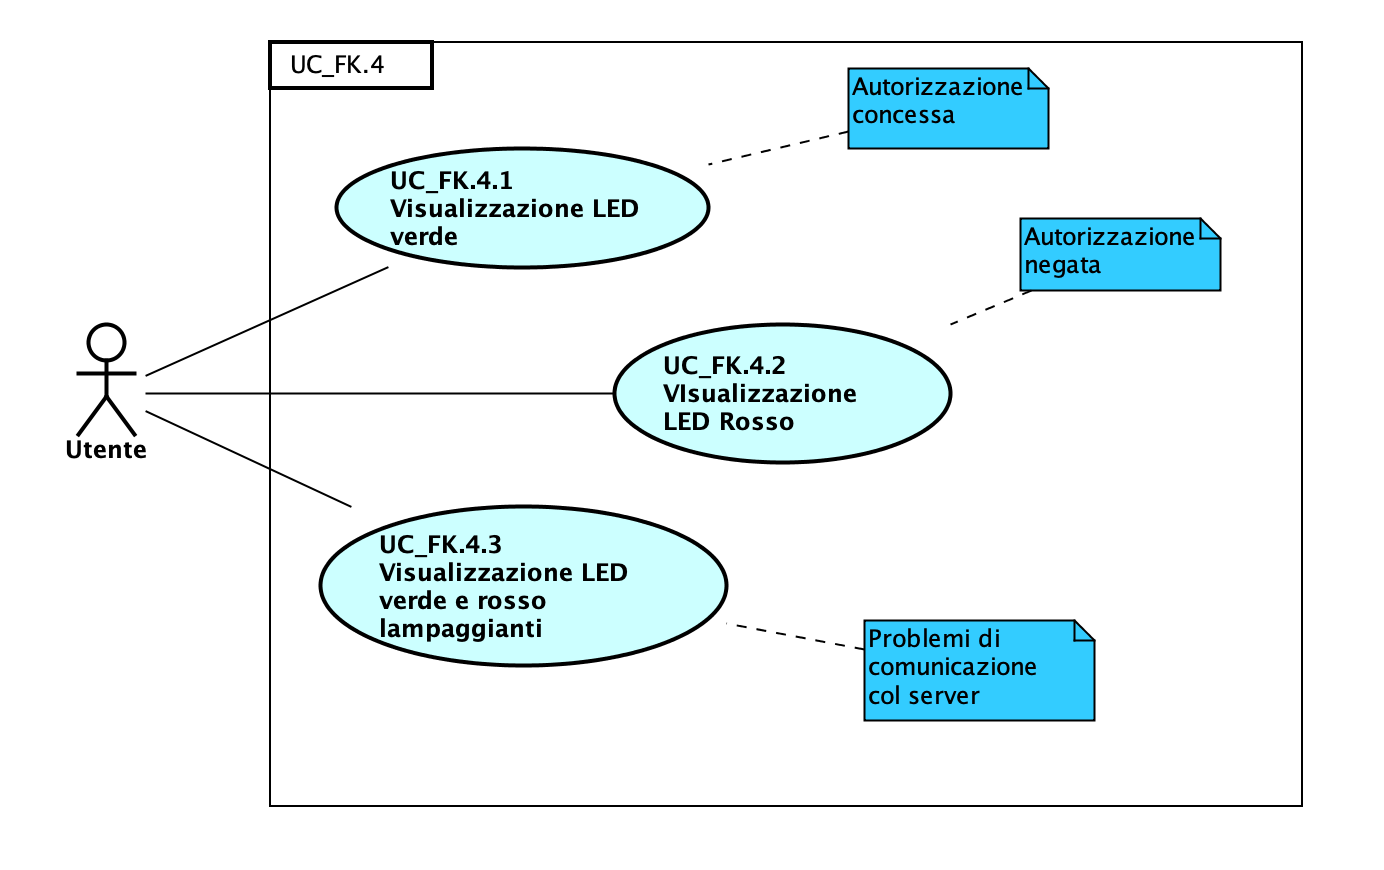
\includegraphics[scale=0.4]{immagini/usecase/UC_FK_4.png}
	\caption{Dettaglio del caso d'uso UC\textunderscore FK.4. Si può notare l'uso della notazione sopra descritta.}
	\end{center}
\end{figure}

Ogni caso d'uso ha una specifica provenienza, ovvero alcune determinate fonti che lo hanno generato.
Queste sono:
\begin{itemize}
\item \textbf{Verbali}: ottenuti trascrivendo quanto emerso durante i colloqui con i portatori di interesse;
\item \textbf{Le specifiche del sistema}: descrivono quali sono le caratteristiche che il sistema deve avere;
\item \textbf{Conoscenza del dominio}: la conoscenza del contesto d'utilizzo e la consultazione di materiale ad esso inerente.
\end{itemize}

Ho utilizzato queste fonti anche per l'identificazione dei requisiti.

\subsection{Formalizzazione dei requisiti}
Dopo aver individuato tutti i requisiti necessari allo sviluppo del progetto, ho creato una codifica che li potesse identificare in maniera univoca e allo stesso tempo catalogare per tipo e priorità.
La codifica utilizzata è la seguente:

\begin{center}
\textbf{R[Componente]\textunderscore [Tipologia]\textunderscore [Priorità][Numero Identificativo]}
\end{center}

\textbf{Componente}
\begin{itemize}
\item \textbf{FK}: requisito inerente allo sviluppo della parte elettronica di FabKey;
\item \textbf{PO}: requisito relativo allo sviluppo del portale online per la gestione degli accessi.
\end{itemize}

\textbf{Tipologia}
\begin{itemize}
\item \textbf{F}: un requisito di tipo funzionale, cioè che aggiunge funzionalità al sistema;
\item \textbf{Q}: requisito di qualità, ovvero che, se soddisfatto, aumenta la qualità generale del prodotto;
\item \textbf{P}: requisito prestazionale, mirato a migliorare il prodotto in termini di prestazioni.
\end{itemize}

\textbf{Priorità}
\begin{itemize}
\item \textbf{Ob}: requisiti obbligatori, il cui sviluppo è condizione necessaria per ottenere il risultato finale;
\item \textbf{De}: requisiti desiderabili, ovvero soddisfarli significa apportare importanti miglioramenti al prodotto anche se non strettamente vincolanti al suo funzionamento;
\item \textbf{Op}: requisiti opzionali, che apportano valore aggiunto al sistema, ma il cui sviluppo è trascurabile.
\end{itemize}

\textbf{Numero Identificativo}

\medskip

Un codice numerico progressivo che identifica in maniera univoca il requisito a cui si riferisce. Questo codice può essere gerarchico.

\bigskip

Riporto di seguito alcuni dei requisiti individuati:

\medskip

\textbf{Hardware FabKey}
\renewcommand{\arraystretch}{2.0}
\begin{longtable}{|l|p{2.5cm}|p{8cm}|}
\hline
\textbf{Codice} & \textbf{Tipo} & \textbf{Descrizione} \\ 
\hline
\textbf{RFK\_F\_Ob1} & Funzionale \linebreak Obbligatorio & Il sistema deve permettere la lettura di un codice a barre \\ 
\hline
\textbf{RFK\_F\_Ob2} & Funzionale \linebreak Obbligatorio & Il sistema deve attivare il lettore quando rileva un utente nelle vicinanze \\
\hline
\textbf{RFK\_Q\_Ob1} & Qualità \linebreak Obbligatorio & Il modulo di lettura deve essere contenuto in un involucro stampato in 3D \\
\hline
\textbf{RFK\_Q\_Op1} & Qualità \linebreak Opzionale & L'involucro esterno deve essere modulare ed espandibile per versioni successive \\
\hline
\caption{Alcuni requisiti individuati per lo sviluppo della parte hardware di FabKey.}
\end{longtable}


\medskip

\textbf{Portale online}
\renewcommand{\arraystretch}{2.0}
\begin{longtable}{|l|p{2.5cm}|p{8cm}|}
\hline
\textbf{Codice} & \textbf{Tipo} & \textbf{Descrizione} \\ 
\hline
\textbf{RPO\_F\_Ob1} & Funzionale \linebreak Obbligatorio & L'applicazione deve permettere di visualizzare l'elenco degli utenti autorizzati \\ 
\hline
\textbf{RPO\_F\_Ob2} & Funzionale \linebreak Obbligatorio & L'applicazione deve permettere di gestire le autorizzazioni \\
\hline
\textbf{RPO\_F\_Ob2.1} & Funzionale \linebreak Obbligatorio & L'applicazione deve permettere di eliminare un'autorizzazione \\
\hline
\textbf{RPO\_F\_De1} & Funzionale \linebreak Desiderabile & L'applicazione deve presentare un'interfaccia grafica completamente scalabile \\
\hline
\caption{Alcuni requisiti individuati per lo sviluppo del gestionale online di FabKey.}
\end{longtable}


Dopo aver individuato e codificato tutti i requisiti, ho composto una tabella in cui ho riportato il tracciamento tra i requisiti e i casi d'uso, in modo da identificare in quale caso d'uso viene soddisfatto un determinato requisito.

\section{Progettazione}
\subsection{L'approccio iniziale}
Ho gestito la progettazione del prodotto in modo separato rispetto alle due componenti principali che ne fanno parte: l'hardware di FabKey (composto da centralina e lettore) e l'applicazione online per la gestione delle autorizzazioni. Per comodità chiamerò queste due componenti \textbf{HWFabKey} e \textbf{Gestionale accessi} rispettivamente.

\medskip

La fase di progettazione è stata molto importante, in quanto la sua corretta realizzazione mi avrebbe permesso una fase di codifica rapida minimizzando i rischi di errore.

\bigskip

\subsection{Progettazione di HWFabKey}

Le componenti alle quali dovevo prestare particolare attenzione durante la fase di progettazione erano quattro:
\begin{itemize}
\item \textbf{Gestione delle componenti elettroniche che compongono il lettore di codice a barre}: durante la progettazione ho ideato lo schema per i collegamenti del lettore di codici a barre (composto da diverse componenti elettroniche), prestando attenzione a non creare interferenze con altre componenti già collegate nella versione esistente, come ad esempio il circuito apri porta;
\item \textbf{Sicurezza nella trasmissione dei dati}: i dati trasmessi verso il server andavano crittografati per evitare di incorrere in alcuni problemi di sicurezza;
\item \textbf{Protocollo di comunicazione con il server}: dovevo scegliere in questa fase il modo in cui la centralina avrebbe comunicato con il server, analizzando pro e contro delle varie alternative.
\item \textbf{Creazione e stampa 3D dell'involucro}: dopo aver abbozzato su carta alcune ipotesi e averne discusso le caratteristiche con il tutor, ho disegnato e stampato in 3D l'involucro;
\end{itemize}

\begin{figure}[H]
	\begin{center}
	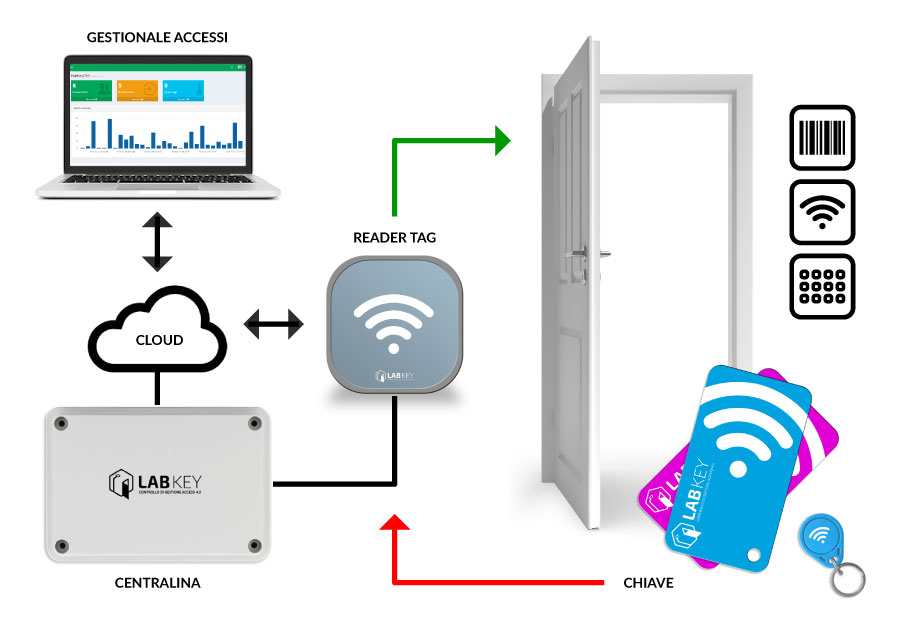
\includegraphics[scale=0.4]{immagini/schema_labkey.jpg}
	\caption{Schema di funzionamento di FabKey.}
	\small{\textbf{Fonte:} \url{https://www.labkey.it}}
	\end{center}
\end{figure}

\subsubsection{Gestione dell'elettronica}
L'utilizzo del nuovo modulo per la lettura di codici a barre ha comportato la gestione di 4 nuove componenti elettroniche, le quali andavano collegate ad Arduino senza interferire con le componenti base del sistema.
Ho risolto tutto questo disegnando lo schema completo ed aiutandomi con un simulatore.

\begin{figure}[H]
	\begin{center}
	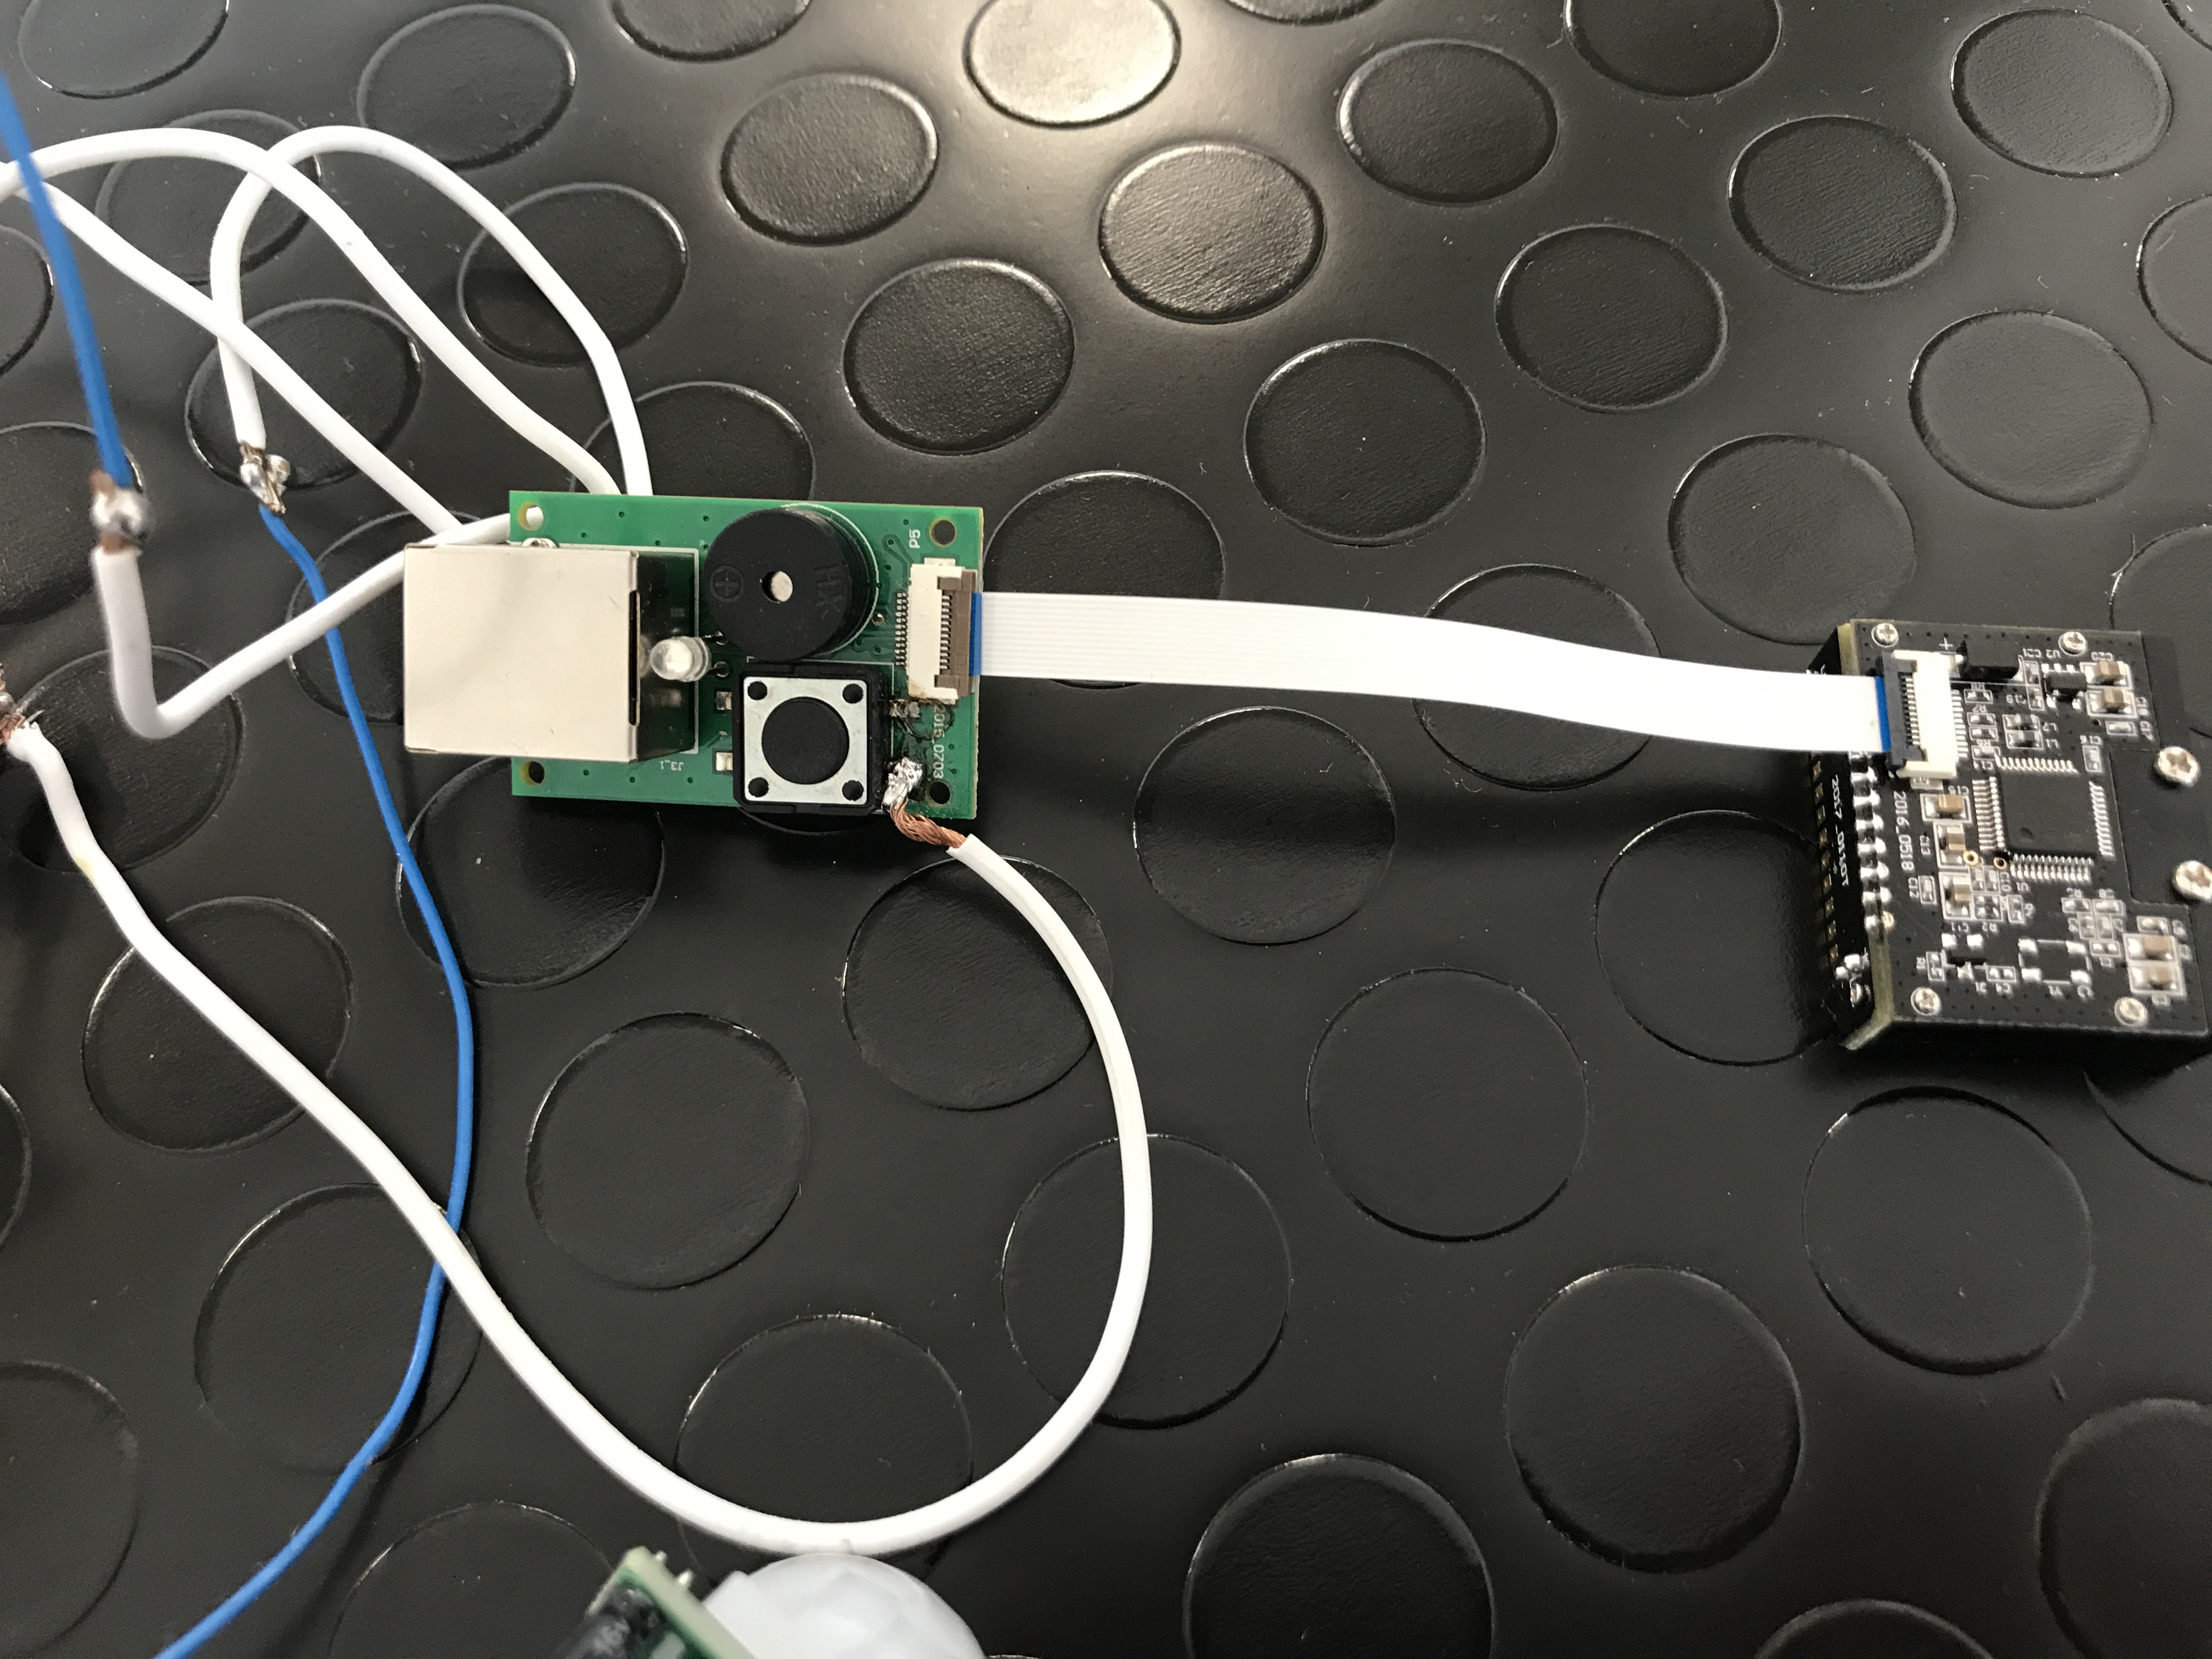
\includegraphics[scale=0.065]{immagini/lettore_barcode.jpg}
	\caption{Una delle componenti elettroniche che compongono il lettore di codici a barre. Si tratta del vero e proprio lettore ottico.}
	\end{center}
\end{figure}

\subsubsection{Sicurezza nella trasmissione dati}
Il maggior problema che ho riscontrato nella gestione della trasmissione dei dati è stato quello riguardante la sicurezza. A primo impatto ho pensato all'uso di una codifica con funzioni crittografiche hash, come ad esempio MD5 o SHA-1, ma non avevo preso in considerazione un aspetto molto importante: la memoria disponibile. 

\begin{figure}[H]
	\begin{center}
	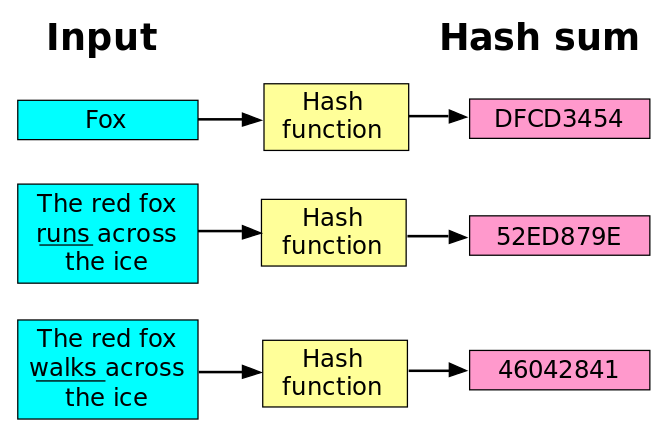
\includegraphics[scale=0.4]{immagini/hash.png}
	\caption{Esempio di funzione hash. Risultato dei primi quattro byte della funzione hash SHA-1.}
	\small{\textbf{Fonte:} \url{https://it.wikipedia.org/wiki/Hash}}
	\end{center}
\end{figure}

Nell'hardware a disposizione le risorse erano estremamente limitate: avevo tralasciato questo aspetto dal momento che ho sempre lavorato con dispositivi la cui potenza di calcolo era trascurabile per questo tipo di operazioni. Nel caso specifico, 2 KB di memoria SRAM non erano sufficienti per la gestione dell'intero programma di controllo e contemporaneamente memorizzare una variabile di 40 byte o più, contenente la stringa con codifica hash. Per cui, collaborando con un collega, abbiamo ideato un algoritmo di crittografia semplificato, basato sul principio della funzione hash, ma in grado di produrre un output nettamente ridotto.


\subsubsection{Protocollo di comunicazione}
Uno dei requisiti prevedeva lo scambio di informazioni tra la centralina di controllo, connessa in rete tramite cavo LAN, e il server centrale, contenente il database con gli accessi autorizzati.
Il compito del team era di soddisfare questo requisito in modo che la comunicazione fosse il più rapida possibile.
La soluzione adottata consiste in una semplice chiamata HTTP verso il server: viene creato un \textit{URL} composto dall'indirizzo del server e il codice di accesso richiesto, codificato tramite l'algoritmo sopra descritto; il server, ricevuta la richiesta, ricava dall'\textit{URL} il codice crittografato e lo confronta con i dati presenti nel database, rispondendo con un segnale positivo o negativo.

\begin{figure}[H]
	\begin{center}
	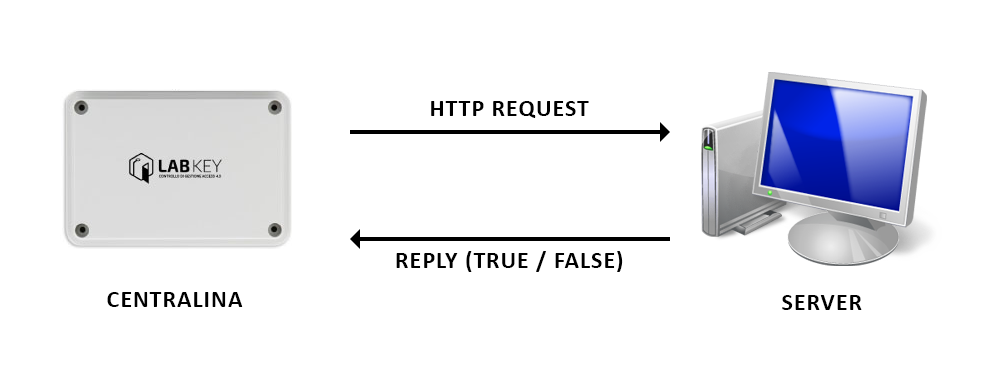
\includegraphics[scale=0.37]{immagini/comunicazione_http.png}
	\caption{Schema di comunicazione Centralina/Server.}
	\end{center}
\end{figure}

\subsubsection{Progettazione dell'involucro e stampa 3D}
L'idea era di realizzare un involucro in grado di contenere tutte le componenti elettroniche del lettore e che fosse allo stesso tempo il più compatto possibile.
Per prima cosa ho abbozzato dei disegni con alcune ipotesi sulle forme generali e, una volta approvato dal tutor, ho iniziato la creazione del modello tridimensionale.

\begin{figure}[H]
	\begin{center}
	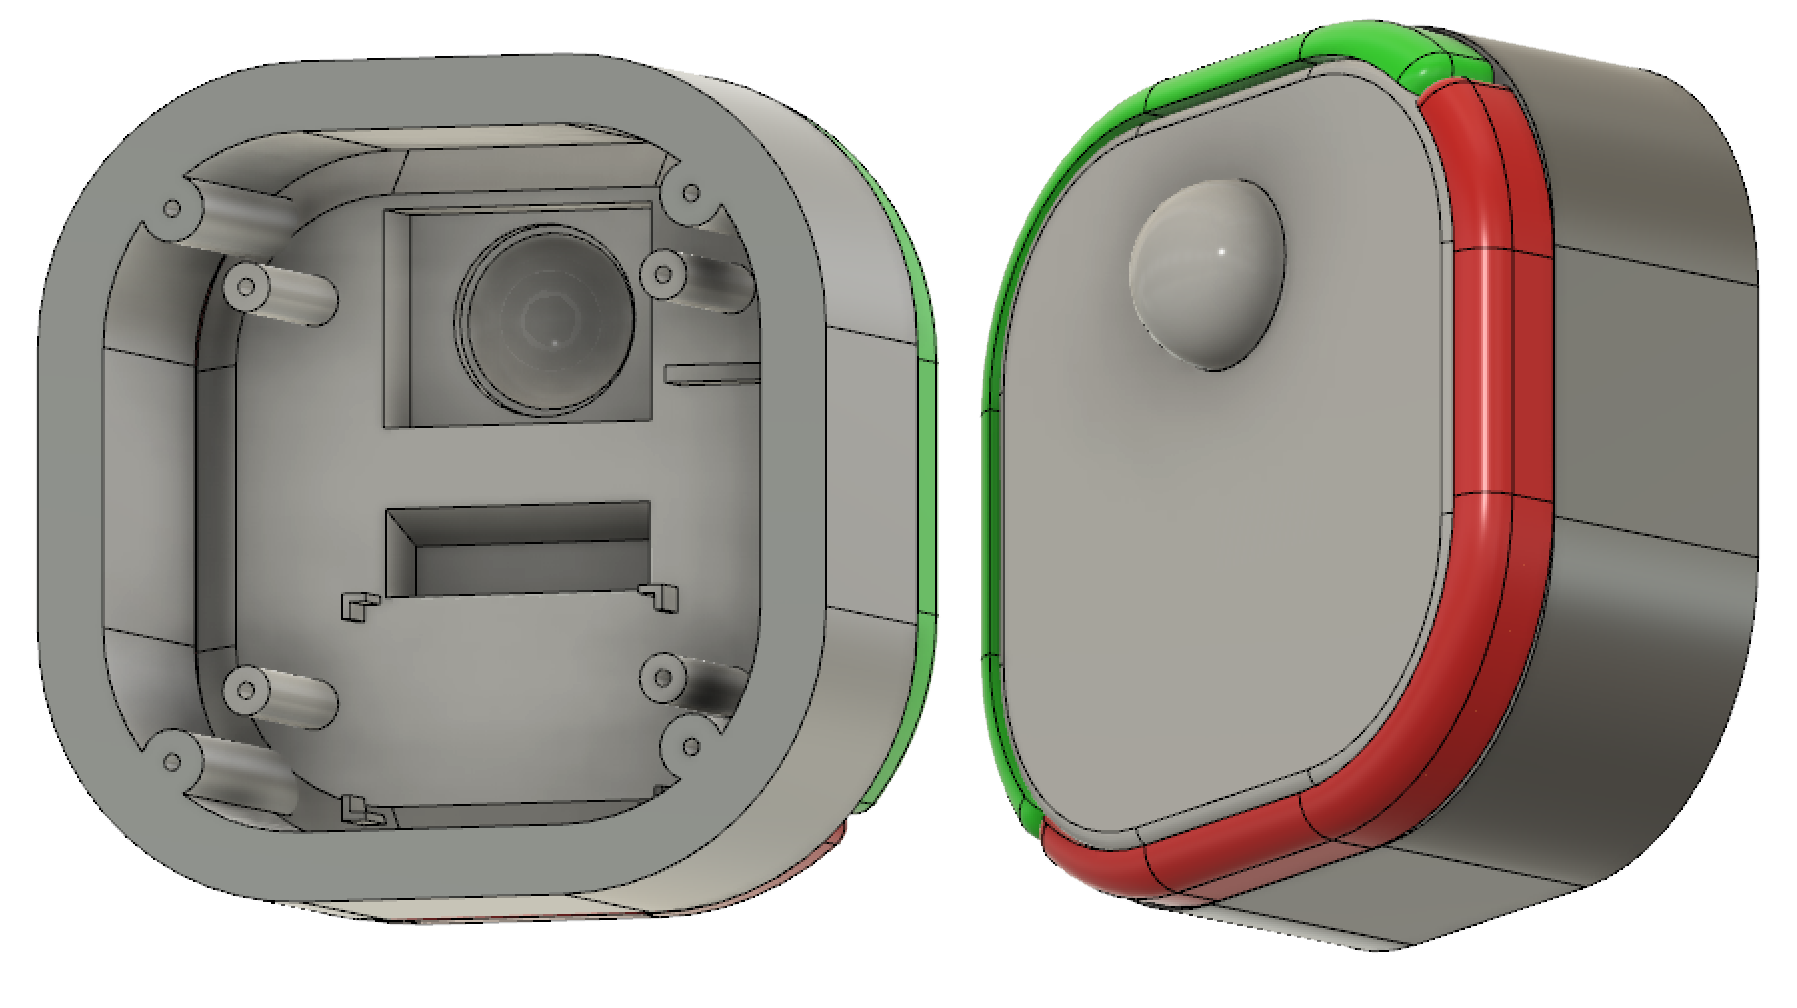
\includegraphics[scale=0.37]{immagini/render.png}
	\caption{La prima versione dell'involucro per il lettore di codici a barre.}
	\end{center}
\end{figure}

Una volta ottenuto il modello finito, ho configurato il processo di stampa grazie al software open source Cura di Ultimaker. Grazie a questa applicazione è possibile, dopo aver impostato i diversi parametri, simulare la stampa, in modo da verificare eventuali errori di configurazione o sul modello.

\begin{figure}[H]
	\begin{center}
	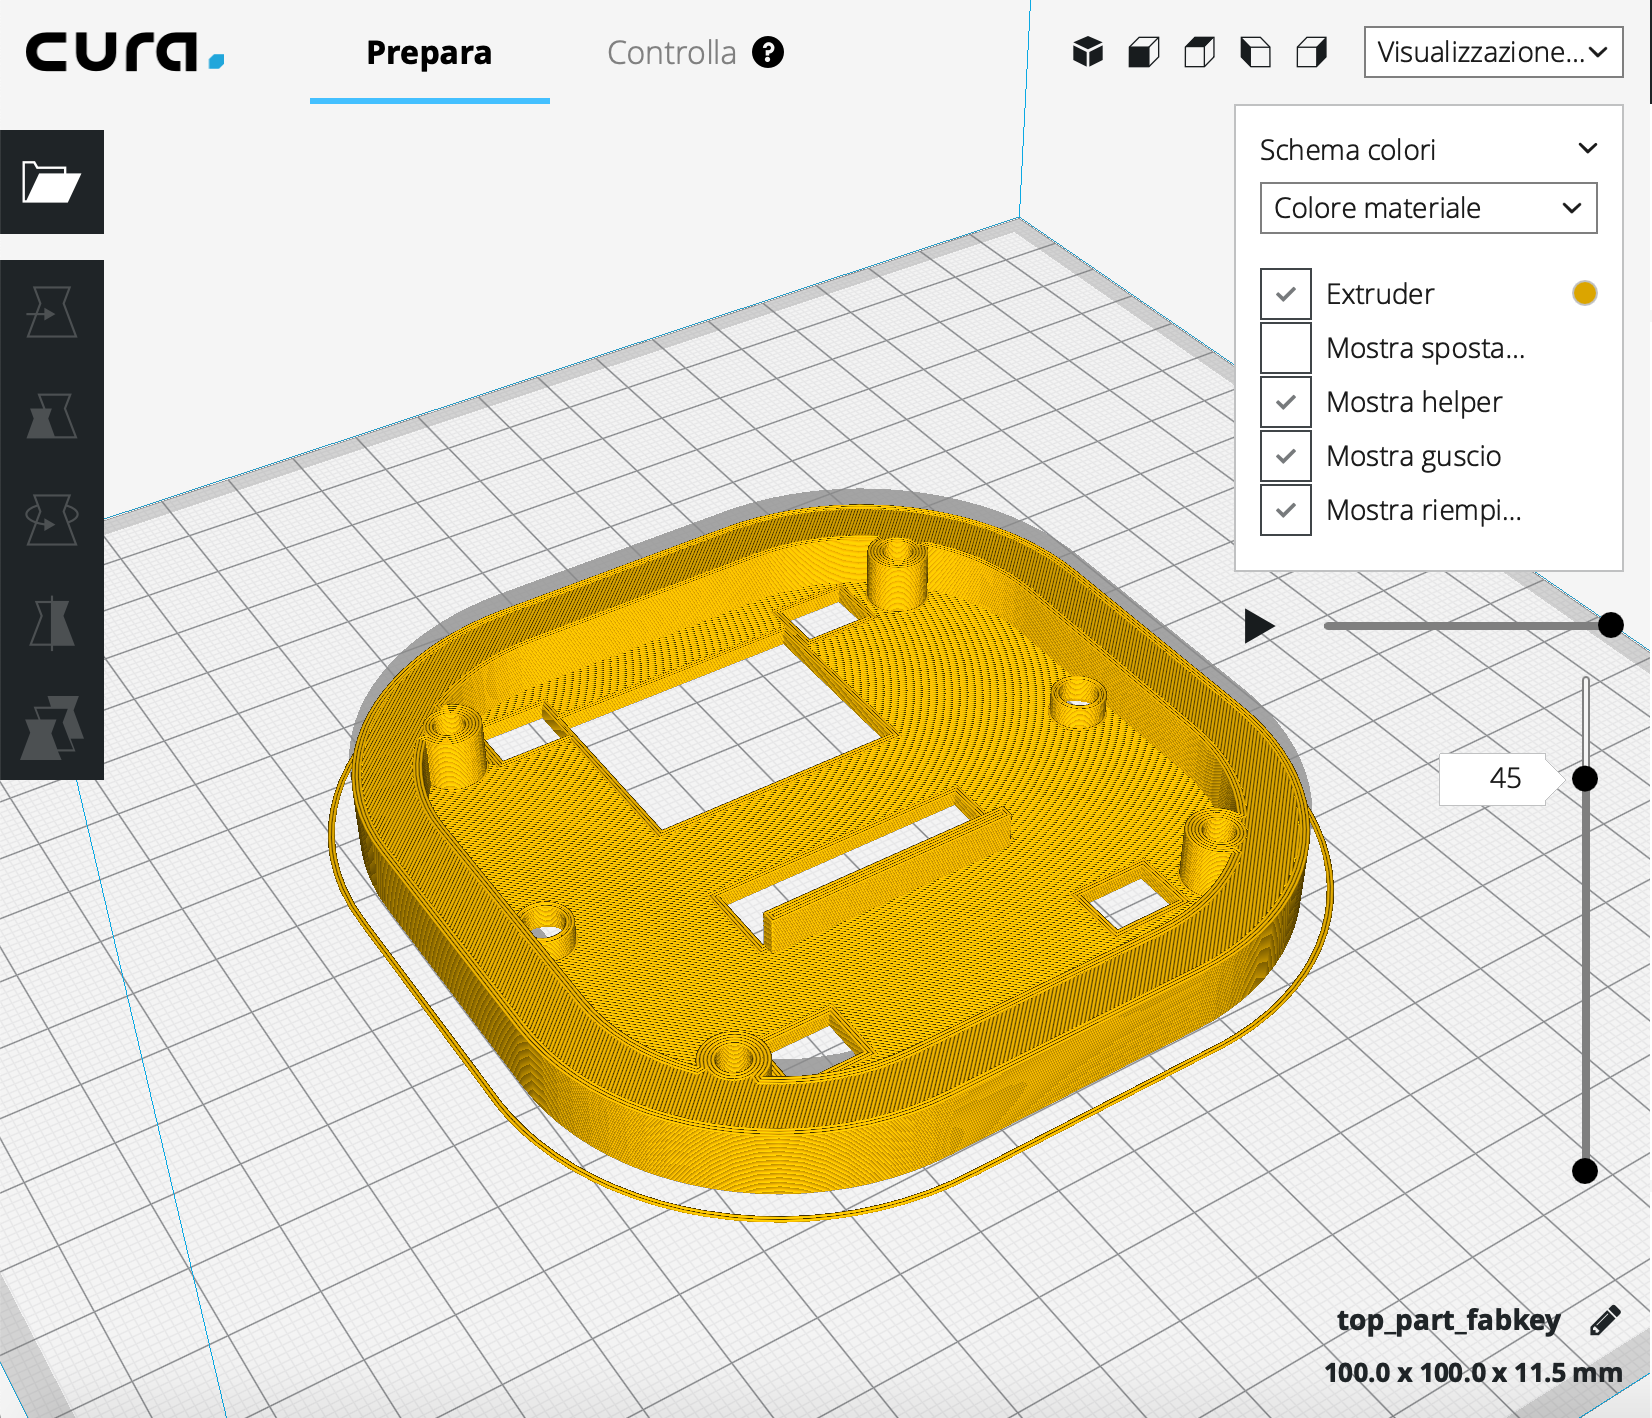
\includegraphics[scale=0.37]{immagini/simulatore_stampa.png}
	\caption{Un componente dell'involucro durante la simulazione con il software Cura.}
	\end{center}
\end{figure}

%Progettazione online app
% Si potrebbe inserire un grafico che rappresenti il database MySql
%ragioni della scelta del db relazionale

\subsection{Progettazione del gestionale accessi}
L'applicazione web per la gestione delle autorizzazioni è composta da un lato front-end e da un lato back-end. La prima parte è formata dall'interfaccia grafica e dalle componenti lato client, mentre la seconda contiene il database e le funzioni per l'elaborazione della risposta alle chiamate http da parte della centralina.

\subsubsection{Front-end - Interfaccia grafica}
Facendo riferimento ai casi d'uso, ho iniziato a progettare l'interfaccia grafica della WebApp, definendo le varie sezioni di cui sarà composta.
Ho previsto un menù di navigazione laterale contenente i collegamenti a tutte le pagine presenti.

\begin{figure}[H]
	\begin{center}
	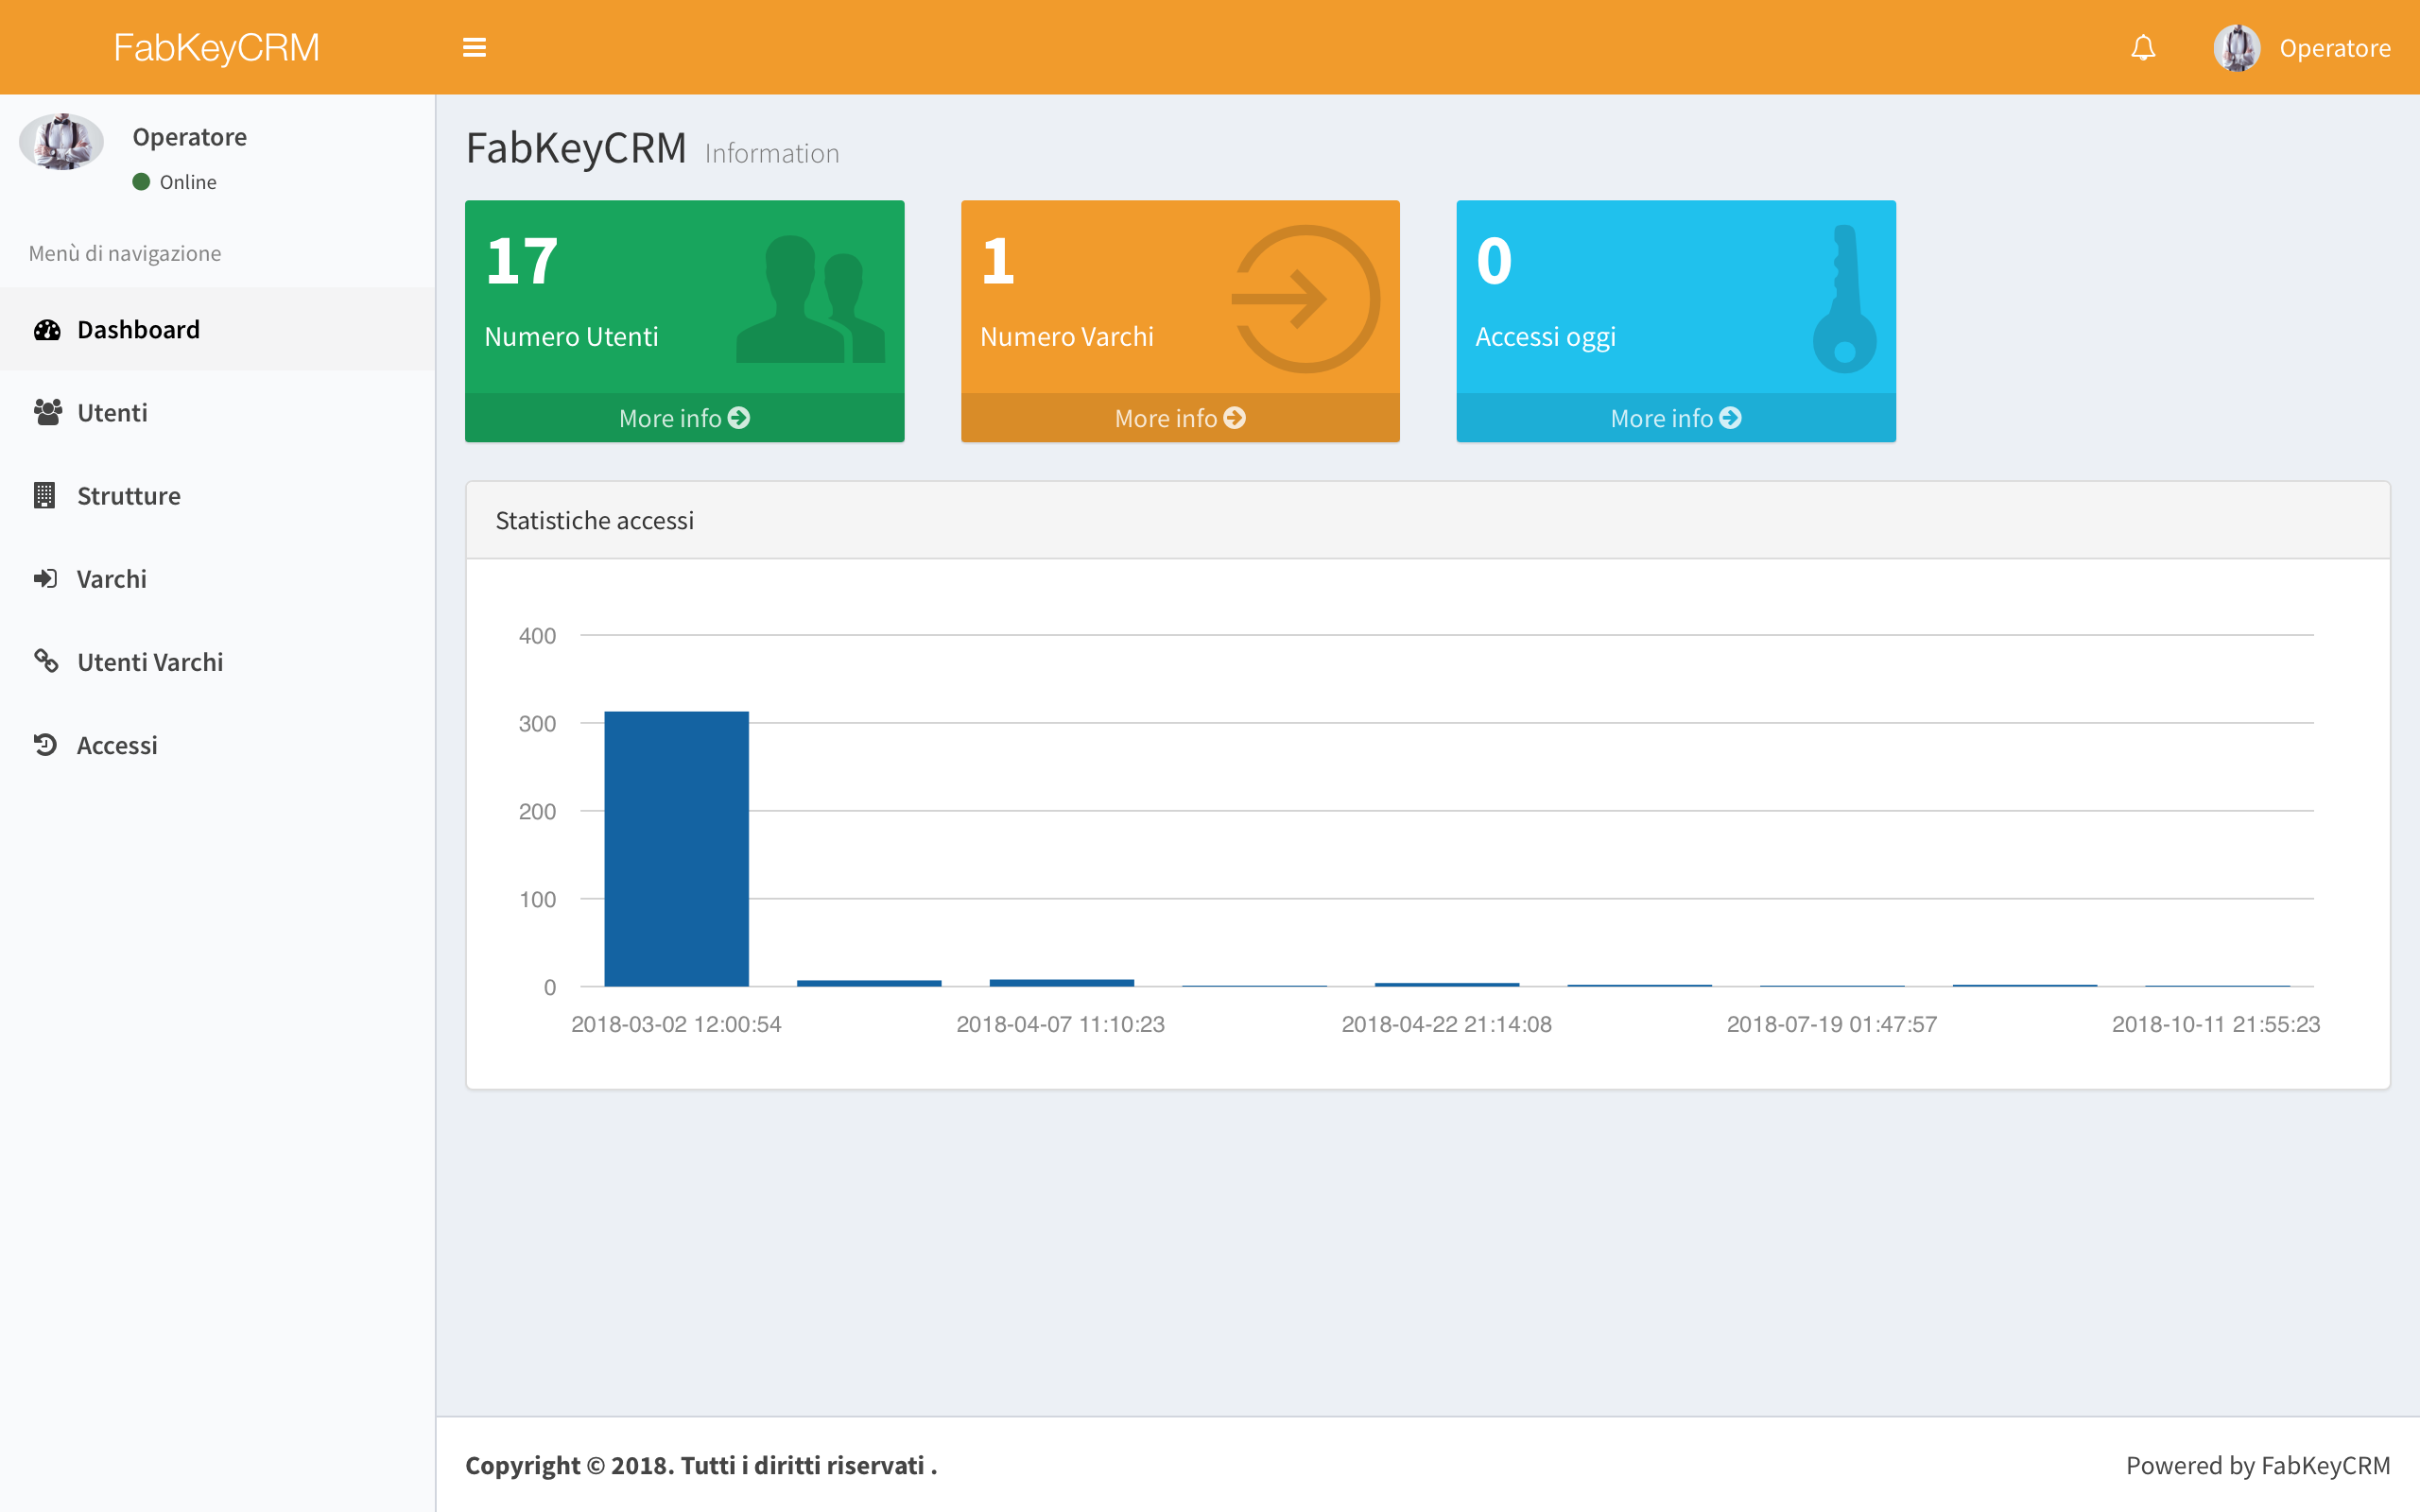
\includegraphics[scale=0.32]{immagini/dashboard_crm.png}
	\caption{Schermata principale del gestionale.}
	\end{center}
\end{figure}

Le sezioni presenti sono:
\begin{itemize}
\item \textbf{Schermata di login}: per poter accedere all'applicazione è necessario collegarsi al sistema con le proprie credenziali ed è possibile effettuarlo in questa schermata;
\item \textbf{Dashboard}: rappresenta la pagina iniziale dopo il login; fornisce all'utente alcune informazioni generali sul sistema, ad esempio il numero di utenti attivi, i varchi, gli accessi effettuati in giornata e una statistica sugli accessi;
\item \textbf{Utenti}: è la pagina che permette la gestione degli utenti con operazioni di inserimento, modifica, eliminazione e assegnazione di una chiave;
\item \textbf{Strutture}: l'applicazione permette tramite questa pagina la gestione di strutture geograficamente dislocate permettendo di aggiungerne di nuove, eliminare le presenti o modificarle;
\item \textbf{Varchi}: i varchi rappresentano le porte di una struttura, pertanto ogni varco è associato ad una struttura;
\item \textbf{Utenti Varchi}: è la sezione che permette di assegnare un utente ad uno o più varchi; in parole povere l'utente può definire quale utente può attraversare determinate porte;
\item \textbf{Accessi}: viene proposto in questa pagina un log degli accessi effettuati con dettagli su utente, varco e orario dell'accesso.
\end{itemize}

\begin{figure}[H]
	\begin{center}
	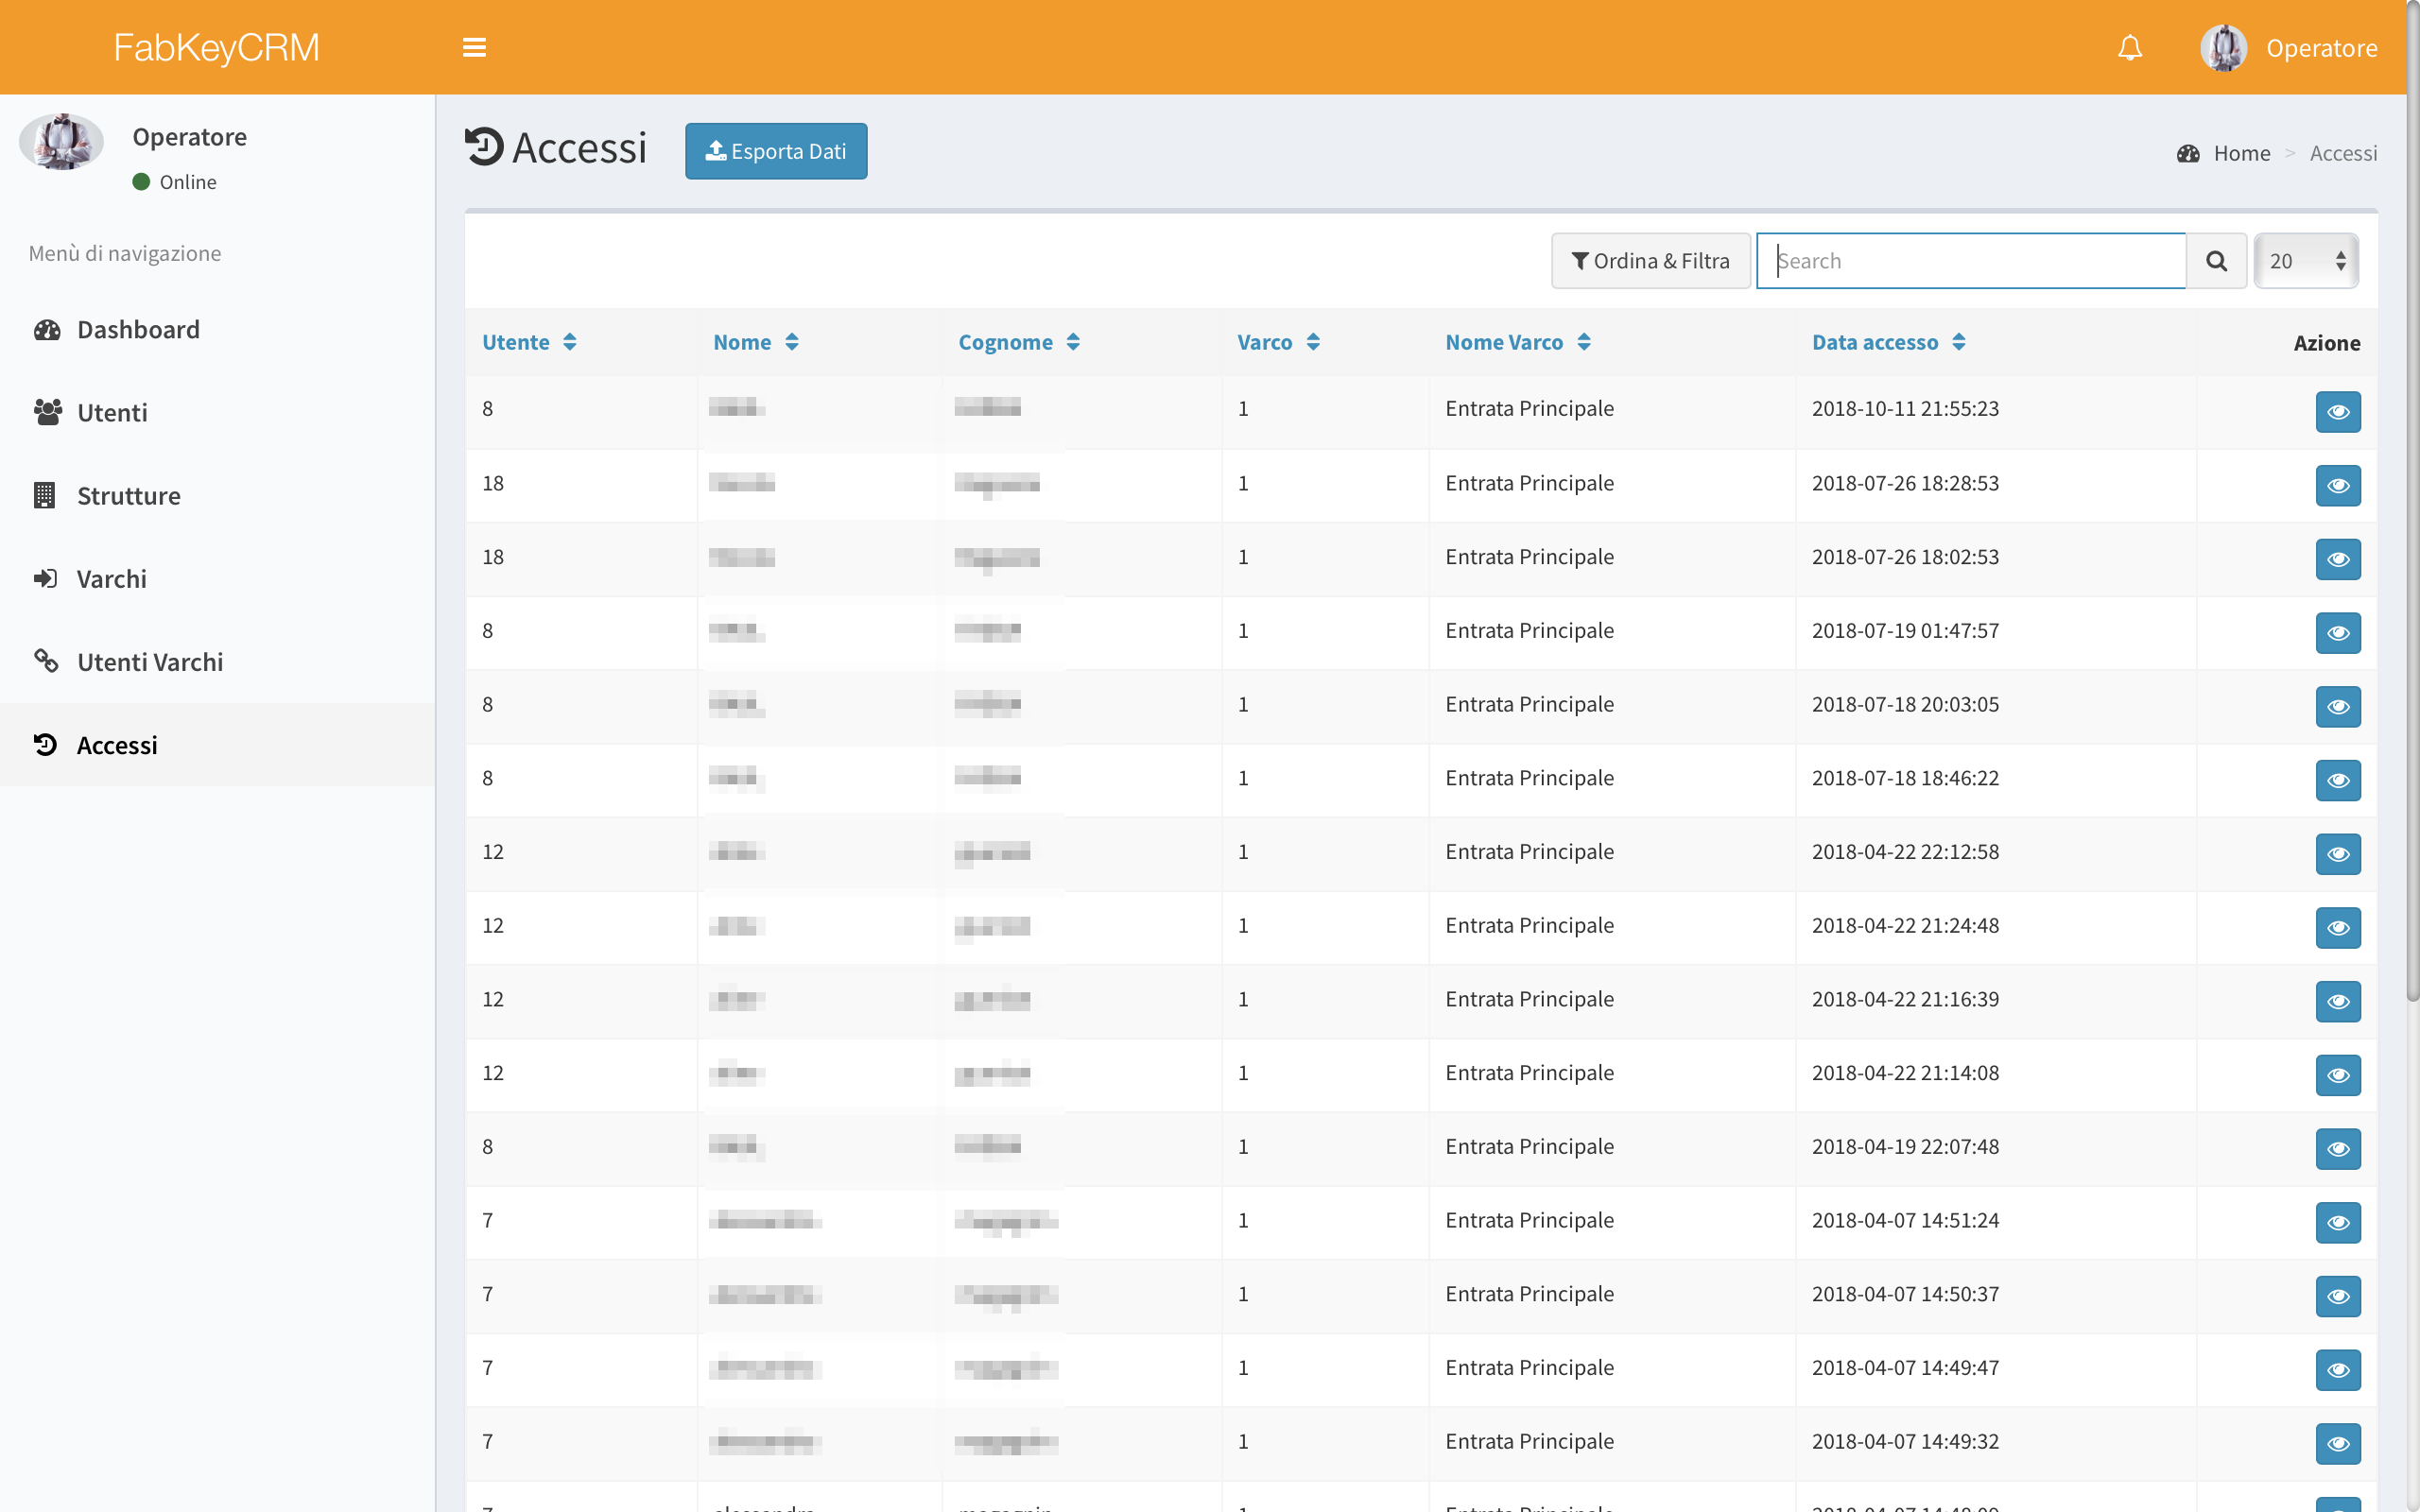
\includegraphics[scale=0.32]{immagini/accessi_crm.png}
	\caption{Schermata del pannello di controllo degli accessi.}
	\end{center}
\end{figure}

\subsubsection{Back-end - Database}
Per la raccolta dei dati abbiamo scelto di creare un database di tipo relazionale SQL.
Ho previsto assieme al team la creazione di tabelle che andassero a rappresentare i vari elementi caratterizzanti del sistema: gli utenti, i varchi, le strutture e alcune tabelle di collegamento per le relazioni di tipo N-N.
Essendo una tecnologia a me già nota, è stata relativamente semplice la progettazione logica del database, portata a termine con il supporto di appositi schemi E-R.

\subsubsection{Back-end - Funzione di risposta}
Parte dell'applicazione è la funzione che gestisce le richieste da parte della centralina. Il principio di funzionamento di questa procedura è relativamente semplice: alla richiesta HTTP della centralina viene estrapolata la chiave crittografata e il varco dal quale è arrivata la richiesta; successivamente si confrontano queste informazioni con i record presenti nel database tramite una query SQL e viene fornita una risposta positiva o negativa. 

\section{Codifica e realizzazione}
\subsection{Tecnologie e linguaggi}
% html, css, javascript, php, mysql, c, bootstrap (o wordpress), librerie Arduino
La fase di codifica consiste nell'implementazione di tutte le componenti definite durante la fase di progettazione, applicando le tecnologie selezionate.

Per prima cosa ho iniziato la codifica della centralina Arduino, le tecnologie coinvolte sono state:

\begin{itemize}
\item \textbf{Arduino IDE e linguaggio C}: per la programmazione del microcontrollore ATMega presente nella scheda Arduino, ho usato l'IDE fornito da Arduino stesso e il linguaggio di programmazione richiesto è il C. Nonostante fossi già ad un buon livello di conoscenza di programmazione con linguaggio C, la trascrizione in codice di quanto progettato non è stata immediata, questo a causa delle diverse librerie da utilizzare, le cui funzioni andavano studiate nel comportamento.
\item \textbf{Librerie Arduino}: ogni particolare componente elettronico disponeva di una specifica libreria per controllarne il funzionamento. Prima di iniziare la codifica finale ho dovuto studiare le funzioni specifiche di queste librerie che sarei andato ad utilizzare.
\begin{itemize}
	\item \textbf{SPI}: \textit{Serial Peripheral Interface} è un protocollo per la comunicazione seriale sincrona usata per la comunicazione tra microcontrollori. Nello specifico ho utilizzato le funzionalità di questa libreria per la comunicazione tra Arduino Uno e il lettore di codici a barre;
	\item \textbf{Ethernet}: la centralina è dotata di un modulo aggiuntivo che la equipaggia di una porta Ethernet. L'apposita libreria per l'utilizzo di questa porta è necessaria per la configurazione di rete;
	
\end{itemize}
\end{itemize}

La traduzione del progetto in codice in questo frangente non è stato per me difficoltoso: ho riscontrato, invece, maggiori problematiche durante la verifica del software, in seguito al caricamento sulla scheda Arduino. Grazie ad alcuni test, ho evidenziato che il codice si comportava saltuariamente in maniera anomala rispetto a quanto previsto, creando un flusso in output apparentemente casuale: ho scoperto in seguito che venivano creati dei caratteri casuali in uscita a causa di interferenze provocate dalla comunicazione seriale con il lettore di codici a barre. Il problema è stato risolto apportando alcune modifiche al software, in modo da ignorare questi caratteri dannosi. I test effettuati sono spiegati nella sezione\textbf{~\ref{test}}.

\medskip

La seconda parte della codifica è stata incentrata sulla creazione del gestionale e le tecnologie utilizzate sono le seguenti:

\begin{itemize}
\item \textbf{PHP e Laravel}: per la codifica della componente back-end del gestionale ho utilizzato il linguaggio PHP con il framework Laravel, caratterizzato da un pattern di tipo Model-View-Controller. Per la gestione del Controller ho sfruttato il supporto fornito da CRUDBooster, un CRUD (Create, Read, Update, Delete) generator che, tramite un sistema a ``scaffolding'', automatizza la creazione di oggetti e interfacce. Queste per me sono state tecnologie nuove e hanno richiesto un periodo di studio individuale precedente alla fase di codifica.
	\begin{itemize}
		\item \textbf{Bootstrap}: è un framework front-end per la creazione di componenti lato client, integrato nel framework Laravel. Ho utilizzato la struttura messa a disposizione da Bootstrap per la creazione delle viste.
	\end{itemize}
\end{itemize}

\subsection{Segnalazione bug e relativa risoluzione}
Non di rado accadeva durante la codifica di riscontrare alcuni bug, oppure di dover integrare alcune caratteristiche al sistema non previste nella progettazione. A questo proposito, durante la fase di progettazione, il team assieme al tutor, aveva concordato una procedura per la gestione di queste situazioni tramite la piattaforma di \textit{GitLab}. Il componente del team che riscontrava un bug o riportava la richiesta di aggiungere nuove funzionalità doveva:
\begin{itemize}
\item Creare un nuovo \textit{issue} fornendo un titolo breve ma esaustivo e una descrizione completa di tutti i dettagli allegando, se necessario, schermate o porzioni di codice. Chi avrebbe letto l'issue avrebbe dovuto essere in grado di interpretarlo senza dover approfondire con chi l'aveva creato;
\item Selezionare un assegnatario, che avrebbe avuto l'onere di risolvere il bug, con la possibilità di assegnare l'issue anche a se stessi;
\item Etichettare l'issue con una o piu \textit{labels}, per identificare il tipo di problema riportato; nel caso di un problema nella codifica andava riportata la label ``bug'', oppure per l'aggiunta di nuove funzionalità ``enhancement'';
\item Eventualmente, era possibile creare un nuovo branch nel caso di aggiunta di nuove funzionalità isolate dal branch master;
\end{itemize}

\subsection{Stampa 3D}

\medskip

Per completare il prodotto ho realizzato il primo prototipo di involucro con la stampante 3D. 

La procedura per la stampa 3D di un modello, come già sperimentato durante lo studio preliminare, consisteva di tre passaggi strettamente sequenziali:
\begin{itemize}
\item \textbf{Pre-riscaldamento e caricamento del materiale}: tramite il pannello di controllo della stampante, dovevo portare in temperatura il piano di stampa a 60 °C e l'ugello di estrusione a 200 °C. Successivamente andava caricato il filamento di materiale che avrei utilizzato per la creazione del modello: le temperature selezionate erano adatte per l'utilizzo di un materiale chiamato PLA (acido polilattico).
\end{itemize}

\begin{figure}[H]
	\begin{center}
	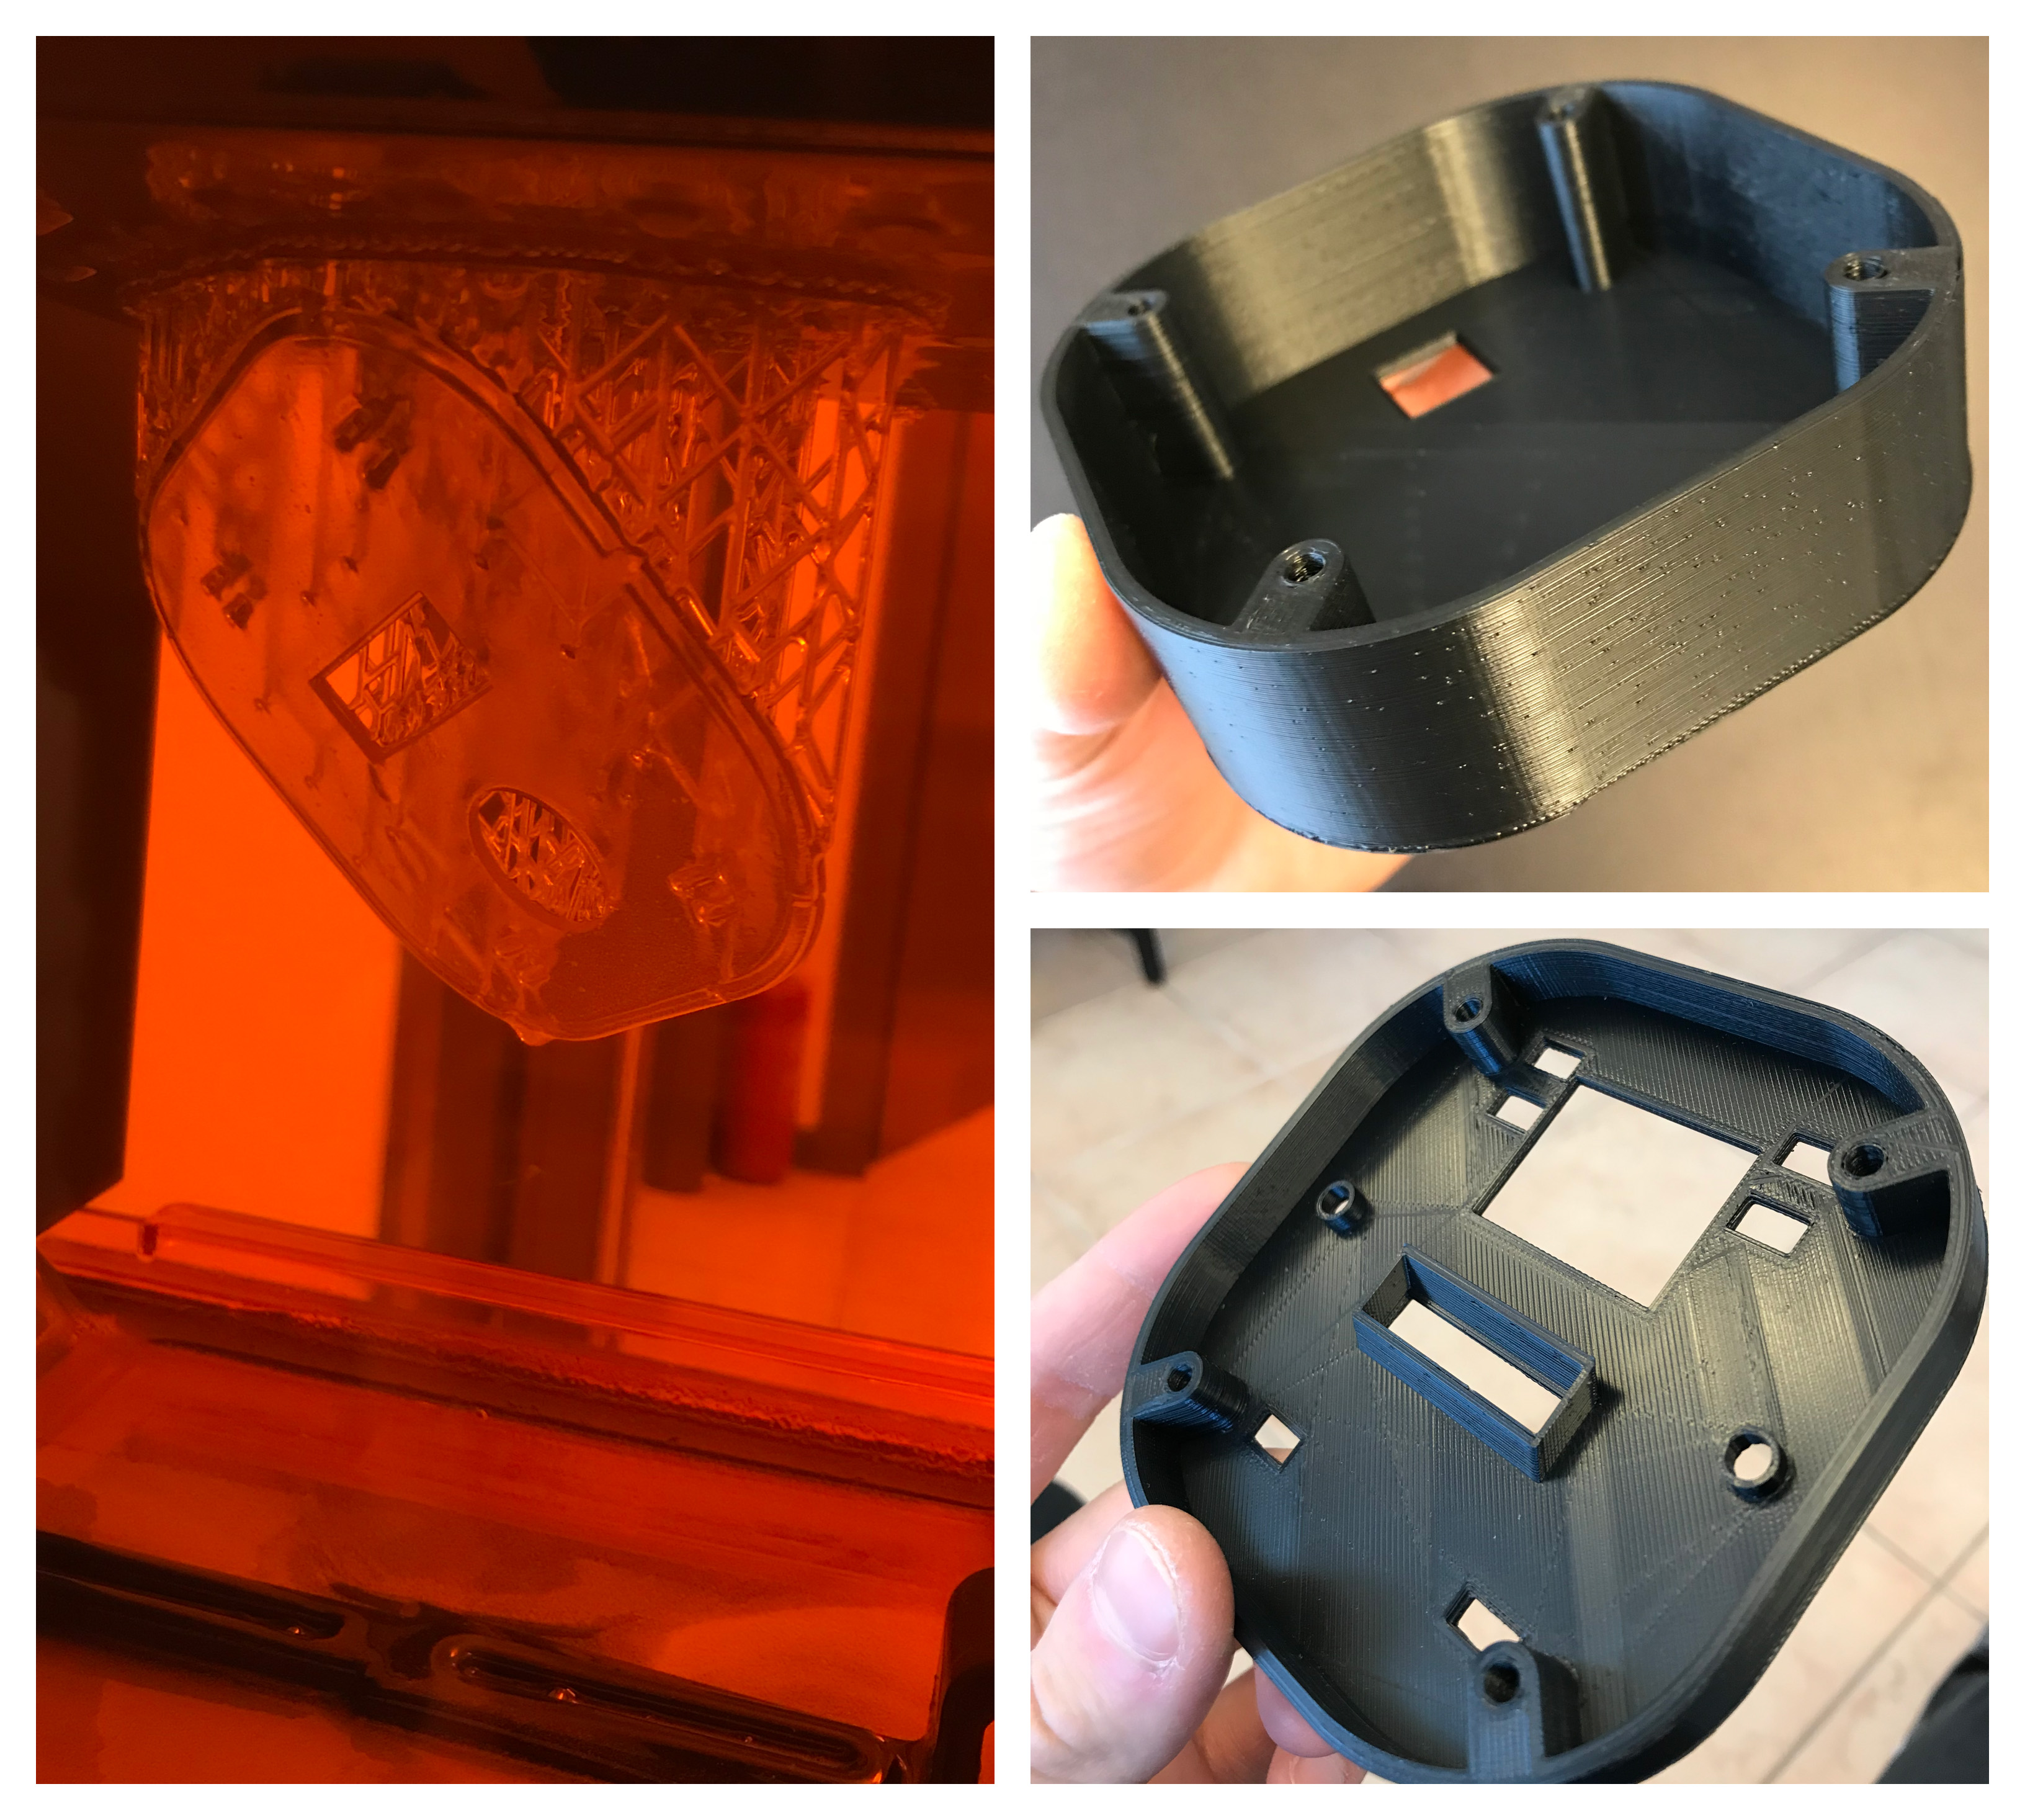
\includegraphics[scale=0.07]{immagini/stampa_3d_finale.png}
	\caption{I primi prototipi di involucro stampati in 3D.}
	\end{center}
\end{figure}

Con l'involucro a disposizione ho potuto procedere con l'assemblaggio finale di tutte le componenti elettroniche, terminando così la prima versione del prodotto. A codifica completata, ho concluso con la preparazione dei test di sistema e successivamente con la loro esecuzione.

\subsection{Redazione dei manuali}
Parte dei requisiti era anche la redazione di tutti i manuali.
In totale ho redatto tre manuali:
\begin{itemize}
\item \textbf{Manuale d'uso utente}: questo manuale è stato scritto per guidare l'utente finale all'utilizzo sia della piattaforma online per la gestione degli utenti, che per l'utilizzo del sistema di apertura porta;
\item \textbf{Manuale di installazione}: breve guida per l'installatore dove sono riportate le istruzioni per la corretta installazione delle componenti elettriche quali centralina e lettore esterno;
\item \textbf{Manuale di configurazione}: questo è un manuale ad uso interno, il suo scopo è di guidare il tecnico durante l'assemblaggio delle componenti elettroniche e la configurazione software, operazioni previste prima della consegna al cliente;
\end{itemize}

Per la scrittura dei manuali ho utilizzato \LaTeX

\section{Verifica e validazione}
\subsection{Test}\label{test}
Al fine di collaudare e validare il prodotto ho previsto diversi test di unità e di sistema per verificare la correttezza di porzioni di codice e la loro integrazione nel sistema completo. I test di unità, a differenza di quelli di sistema, sono stati eseguiti anche durante la fase di codifica, in modo da segnalare ed eliminare tempestivamente la presenza di eventuali bug.
\subsubsection{Test del codice di Arduino}
Effettuare dei test di unità direttamente sulla scheda Arduino avrebbe dato vita ad un processo ripetitivo e lento composto da:
\begin{itemize}
\item Modifica del codice;
\item Compilazione e caricamento sulla scheda Arduino;
\item Osservazione del comportamento e trarre ipotesi sul suo funzionamento, positivo o negativo che sia;
\item Ripetere i passaggi.
\end{itemize}

Per questo motivo ho deciso di testare la qualità del codice scritto facendolo eseguire direttamente al computer. 
I test di unità che ho previsto avevano la seguente struttura:
\begin{enumerate}
\item Per prima cosa ho isolato la parte di codice di interesse, rendendola eseguibile come programma esterno;
\item Ho composto una previsione di output anche relazionata all'eventuale input fornito all'unità;
\item Nel caso in cui la porzione di codice effettuasse chiamate a funzioni di librerie esterne, ho creato dei mock-up che avrebbero simulato il comportamento di tali procedure, in modo da testare esclusivamente la qualità del codice scritto da me;
\item Dopo l'esecuzione del test, se l'output corrispondeva alle attese si procedeva al caricamento del test sulla scheda Arduino, altrimenti si modificava il codice in modo da correggerlo;
\item Se il comportamento del codice eseguito sulla scheda Arduino era ancora corretto, il test terminava, altrimenti si procedeva identificando e correggendo la natura del comportamento anomalo.
\end{enumerate}

\begin{figure}[H]
	\begin{center}
	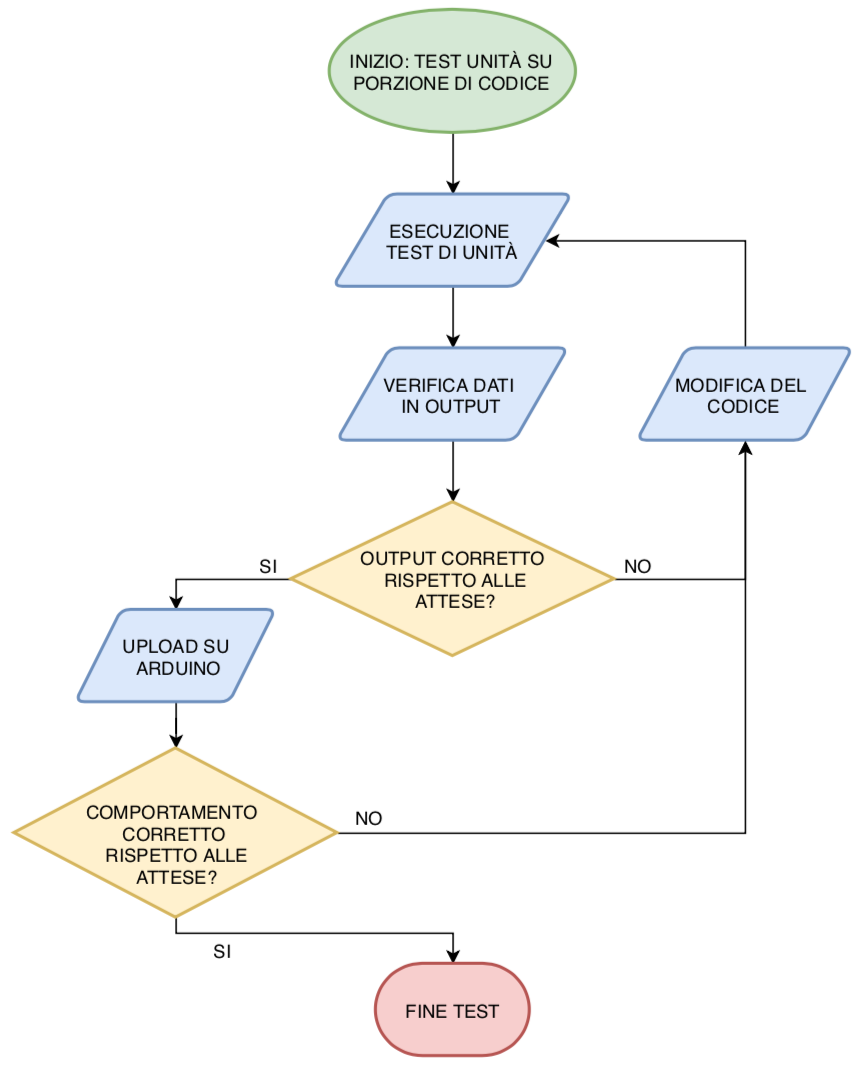
\includegraphics[scale=0.6]{immagini/flow_chart.png}
	\caption{Diagramma rappresentante l'esecuzione di un test di unità.}
	\end{center}
\end{figure}

Con questa procedura ho riscontrato, come atteso, che circa nel 90\% dei casi la porzione di codice aveva lo stesso comportamento sia nell'esecuzione sul computer che sulla scheda Arduino. In questo modo ho ridotto i tempi ottimizzando il processo di test.

\subsubsection{Test gestionale utente}
Parallelamente ad Arduino, e quindi alla centralina, dovevo eseguire dei test anche sulla piattaforma online di gestione degli accessi.
Anche in questo caso ho previsto alcuni test di unità sul codice PHP che gestisce la parte dinamica dell'applicazione. Per farlo ho utilizzato il framework di testing PHPUnit, incluso nel framework Laravel; ho isolato singolarmente le funzionalità implementate oggetto di test e, per ognuna di queste, scritto degli snippet per simularne il funzionamento sia in condizioni normali che anomale.

Laravel mette inoltre a disposizione un API di semplice utilizzo per effettuare chiamate HTTP e verificare l'output di tali chiamate. Ho utilizzato queste funzionalità per testare l'applicazione in tutte le sue parti, simulando l'utilizzo da parte di un utente, ma ho anche testato la funzione che gestisce le chiamate HTTP da parte della centralina, simulando l'invio di alcune chiavi e analizzando la risposta del server.

\medskip

Per l'occasione ho creato un file di configurazione dedicato alla fase di test del tipo \verb|.env.testing|, e un database separato, già popolato con dati utili.

\medskip

Di seguito uno dei test eseguiti per analizzare l'efficacia delle chiamate HTTP dalla centralina Arduino verso il server:

\definecolor{bg}{RGB}{240,243,243}
\usemintedstyle{manni}% Ref test Laravel: https://blog.pusher.com/tests-laravel-applications/
\inputminted[bgcolor=bg, frame=lines, framesep=2mm, startinline=true, breaklines=true, fontsize=\small, linenos=true]{php}{capitoli/code.php}

Il codice sopra riportato simula l'invio di una chiave cifrata, corrispondente ad un utente con permesso di accesso. Se il test fallisce significa che i valori di risposta ottenuti non corrispondono alle attese; al contrario, se il test termina correttamente, l'unità di codice è stata verificata con successo.

\subsubsection{Riepilogo finale}
Al termine dell'esecuzione dei test ho potuto trarre delle conclusioni rispetto alla copertura di codice per quanto riguarda i test di unità e alla copertura dei requisiti per i test di sistema.

\medskip

I test di unità mi sono tornati utili per poter dimostrare la correttezza e la completezza del codice scritto, analizzando porzioni di codice, nella maggior parte dei casi identificate da procedure. Di seguito i risultati di tali test:

\renewcommand{\arraystretch}{1.2}
\begin{longtable}{|p{2.7cm}|l|l|l|}
\hline
\textbf{Applicazione} & \textbf{Test eseguiti} & \textbf{Test superati} & \textbf{Copertura} \\ 
\hline
\textbf{HWFabKey} & 18 & 18 & 69\%\\ 
\hline
\textbf{Gestionale accessi front-end} & 24  & 24 & 72\%\\ 
\hline
\textbf{Gestionale accessi back-end} & 33  & 33 & 78\%\\ 
\hline
\caption{Risultati dei test di unità.}
\end{longtable}

I test di sistema, invece, mi hanno permesso di verificare la copertura dei requisiti, confrontando quelli definiti durante la fase di analisi con quelli sviluppati al termine del progetto. Di seguito i risultati:

\begin{longtable}{|p{2.7cm}|l|l|}
\hline
\textbf{Test eseguiti} & \textbf{Requisiti definiti} & \textbf{Requisiti soddisfatti} \\ 
\hline
11 & 31 & 29\\ 
\hline
\caption{Risultati dei test di sistema.}
\end{longtable}

\subsubsection{Collaudo finale e consegna}
Al seguito di tutti i test, io e il tutor abbiamo organizzato un collaudo finale convocando il cliente che avrebbe effettuato la prima installazione del prodotto. Il collaudo finale si è svolto simulando tutte le operazioni previste e dimostrando la copertura completa di tutti i requisiti richiesti in fase di analisi.
La dimostrazione si è conclusa senza imprevisti e con la soddisfazione del cliente, inoltre io, il tutor e il cliente abbiamo firmato un verbale di collaudo che constatava la fine dello sviluppo del progetto e dava la possibilità di procedere con la prima installazione.

%\section{Visione generale del progetto}             % Lo stage
% !TEX encoding = UTF-8
% !TEX TS-program = pdflatex
% !TEX root = ../tesi.tex

%**************************************************************
\chapter{Valutazione retrospettiva}
\label{cap:valutazione-retrospettiva}
%**************************************************************

\section{Obiettivi raggiunti}
%Breve bilancio sugli obiettivi raggiunti in rapporto a quelli preventivati.
Al termine del progetto di stage ho analizzato gli obiettivi raggiunti rispetto a quelli fissati inizialmente. Di seguito riporto una tabella con le valutazioni.

\renewcommand{\arraystretch}{2.0}
\begin{longtable}{|p{7cm}|p{2.5cm}|p{3cm}|}
\hline
\textbf{Obiettivo} & \textbf{Tipo} & \textbf{Esito finale} \\ 
\hline
\textbf{Integrazione di un sistema completo per l'apertura di serrature con lettura di codice a barre e NFC} & Obbligatorio & Soddisfatto \\ 
\hline
\textbf{Realizzazione della piattaforma web per la gestione degli accessi} & Obbligatorio & Soddisfatto \\ 
\hline
\textbf{Creazione del modello 3D dell'involucro e sua realizzazione con stampa 3D} & Obbligatorio & Soddisfatto \\ 
\hline
\textbf{Redazione della manualistica completa} & Obbligatorio & Soddisfatto \\ 
\hline
\textbf{Cura e definizione dell'interfaccia grafica della piattaforma web} & Desiderabile & Soddisfatto \\ 
\hline
\textbf{Ottimizzazione del sistema esistente in termini di efficienza e prestazioni} & Desiderabile & Non soddisfatto \\ 
\hline
\textbf{Creazione di un modello 3D modulare espandibile per future versioni} & Facoltativo & Non soddisfatto \\ 
\hline
\caption{Valutazione finale sugli obiettivi aziendali.}
\end{longtable}

\section{Valutazione formativa}
Valutazione di quanto effettivamente appreso durante l'esperienza di stage.

\section{Considerazioni personali}
Analisi sulla distanza (o vicinanza) tra il corso di studi (e quindi le conoscenze apprese durante lo studio) e il mondo lavorativo incontrato durante lo stage, mettendo in evidenza le lacune che si sono dovute colmare per completare il tirocinio.
Consigli al corso di studi sulla base dell'esperienza personale.             % Valutazione retrospettiva
\appendix                               
\input{capitoli/capitolo-A}             % Appendice A

%**************************************************************
% Materiale finale
%**************************************************************
\backmatter
%\printglossaries                   % DA ABILITARE PER IL GLOSSARIO
\input{inizio-fine/bibliografia}
\end{document}